%% mini_project_report.tex — NITK M.Tech Mini Project Report
%% Project: Interpretable and Uncertainty-Aware Crop Price Forecasting
%% Author:  Devulapalli Tharun (252CS009), M.Tech CSE, NITK Surathkal
%% Guide:   Prof. Shashidhar G. Koolagudi

\documentclass[12pt,a4paper]{report}

\usepackage[top=1in,bottom=1in,left=1.25in,right=1in]{geometry}
\usepackage[T1]{fontenc}
\usepackage[utf8]{inputenc}
\usepackage{lmodern}
\usepackage{graphicx}
\usepackage{booktabs}
\usepackage{tabularx}
\usepackage{array}
\usepackage{float}
\usepackage{amsmath}
\usepackage{amssymb}
\usepackage{bm}
\usepackage{caption}
\usepackage{titlesec}
\usepackage{indentfirst}
\usepackage{xurl}
\usepackage[hidelinks]{hyperref}
\usepackage{xcolor}
\usepackage{tikz}
\usetikzlibrary{arrows.meta,positioning,shapes.geometric,calc}

%% -- Colours for TikZ diagrams --
\definecolor{cdata}{HTML}{E0F7FA}
\definecolor{cdataborder}{HTML}{006064}
\definecolor{cfeat}{HTML}{E8F5E9}
\definecolor{cfeatborder}{HTML}{1B5E20}
\definecolor{cmodel}{HTML}{FFF3E0}
\definecolor{cmodelborder}{HTML}{BF360C}
\definecolor{ccalib}{HTML}{FFFDE7}
\definecolor{ccalibborder}{HTML}{F57F17}
\definecolor{cdeploy}{HTML}{ECEFF1}
\definecolor{cdeployborder}{HTML}{37474F}
\definecolor{cvsn}{HTML}{F3E5F5}
\definecolor{cvsnborder}{HTML}{4A148C}
\definecolor{clstm}{HTML}{E8EAF6}
\definecolor{clstmborder}{HTML}{1A237E}
\definecolor{cattn}{HTML}{FCE4EC}
\definecolor{cattnborder}{HTML}{880E4F}

%% -- Chapter/section title formatting --
\titleformat{\chapter}[hang]
    {\normalfont\LARGE\bfseries}
    {\thechapter}{1em}{}
\titlespacing*{\chapter}{0pt}{40pt}{20pt}

\titleformat{\section}
    {\normalfont\large\bfseries}
    {\thesection}{1em}{}
\titlespacing*{\section}{0pt}{12pt}{6pt}

\titleformat{\subsection}
    {\normalfont\normalsize\bfseries}
    {\thesubsection}{1em}{}
\titlespacing*{\subsection}{0pt}{8pt}{4pt}

\titleformat{\subsubsection}
    {\normalfont\normalsize\bfseries}
    {\thesubsubsection}{1em}{}
\titlespacing*{\subsubsection}{0pt}{6pt}{2pt}

\renewcommand{\contentsname}{Contents}
\captionsetup{font=small, labelsep=colon, labelfont=bf}

\newcolumntype{L}[1]{>{\raggedright\arraybackslash}p{#1}}
\setcounter{secnumdepth}{3}
\setcounter{tocdepth}{2}
\setlength{\emergencystretch}{3em}

\begin{document}
\hypersetup{pageanchor=false}

%% =====================================================================
%% TITLE PAGE
%% =====================================================================
\begin{titlepage}
\centering
\vspace*{1.2cm}

{\LARGE\bfseries Interpretable and Uncertainty-Aware Crop Price}\\[0.4em]
{\LARGE\bfseries Forecasting for Indian Markets using}\\[0.4em]
{\LARGE\bfseries Temporal Fusion Transformers}

\vspace{1.4cm}
{\normalsize Mini Project Report}

\vspace{0.8cm}
{\normalsize\itshape Submitted in partial fulfillment of the requirements for the degree of}

\vspace{0.5cm}
{\large\bfseries Master of Technology in Computer Science and Engineering}

\vspace{0.5cm}
{\normalsize\itshape by}

\vspace{0.5cm}
{\large\bfseries Devulapalli Tharun (252CS009)}

\vspace{1.2cm}
{\normalsize\itshape under the guidance of}

\vspace{0.5cm}
{\large\bfseries Prof. Shashidhar G. Koolagudi}

\vspace{1.4cm}

\IfFileExists{figures/NITK_Emblem.png}{%
    
\includegraphics[height=4cm]{figures/NITK_Emblem.png}%
}{%
    \textbf{[NITK EMBLEM]}%
}

\vspace{1.4cm}

{\normalsize DEPARTMENT OF COMPUTER SCIENCE AND ENGINEERING\\[0.3em]
NATIONAL INSTITUTE OF TECHNOLOGY KARNATAKA,\\[0.3em]
SURATHKAL, MANGALORE -- 575025\\[0.5em]
May, 2026}

\end{titlepage}

%% =====================================================================
%% BLANK PAGE
%% =====================================================================
\clearpage
\thispagestyle{empty}
\phantom{x}
\clearpage

%% =====================================================================
%% DECLARATION
%% =====================================================================
\thispagestyle{empty}
\vspace*{1.5cm}
\noindent\fbox{%
\begin{minipage}{\dimexpr\textwidth-2\fboxsep-2\fboxrule\relax}
\vspace{1cm}

\begin{center}
\textbf{DECLARATION}
\end{center}

\vspace{1cm}

\hspace{\parindent}I hereby declare that the \textbf{Mini Project} report entitled \textbf{Interpretable and Uncertainty-Aware Crop Price Forecasting for Indian Markets using Temporal Fusion Transformers} being submitted to the Department of Computer Science and Engineering, National Institute of Technology Karnataka, Surathkal, in fulfilment of the requirements of the M.Tech in CSE is a bona fide report of the work carried out by me. The material contained in this Report has not been submitted to any University or Institution for the award of any degree.

\vspace{2.5cm}

\hfill
\begin{minipage}{0.5\textwidth}
Devulapalli Tharun (252CS009)\\
Department of Computer Science and Engineering\\
NITK, Surathkal
\end{minipage}

\vspace{2cm}

\noindent Place: NITK, Surathkal.\\
Date: 04-05-2026

\vspace{0.8cm}
\end{minipage}%
}
\clearpage

%% =====================================================================
%% BLANK PAGE
%% =====================================================================
\thispagestyle{empty}
\phantom{x}
\clearpage

%% =====================================================================
%% CERTIFICATE
%% =====================================================================
\thispagestyle{empty}
\vspace*{1.5cm}
\noindent\fbox{%
\begin{minipage}{\dimexpr\textwidth-2\fboxsep-2\fboxrule\relax}
\vspace{1cm}

\begin{center}
\textbf{CERTIFICATE}
\end{center}

\vspace{1cm}

\hspace{\parindent}This is to certify that the \textbf{Mini Project} report entitled \textbf{Interpretable and Uncertainty-Aware Crop Price Forecasting for Indian Markets using Temporal Fusion Transformers} submitted by \textbf{Devulapalli Tharun (252CS009)}, as the record of the work carried out, is accepted as the Mini Project work report submission in partial fulfillment for the award of the degree of Master of Technology in Computer Science and Engineering in the Department of Computer Science and Engineering, NITK, Surathkal.

\vspace{3.5cm}

\noindent\textbf{Signature of Project Guide with date}\\[0.4em]
Prof. Shashidhar G. Koolagudi,\\
Department of Computer Science and Engineering,\\
NITK, Surathkal

\vspace{1.5cm}
\end{minipage}%
}
\clearpage

%% =====================================================================
%% FRONT MATTER
%% =====================================================================
\pagenumbering{roman}
\setcounter{page}{1}
\thispagestyle{plain}
\phantom{x}
\clearpage

%% =====================================================================
%% ABSTRACT
%% =====================================================================
\chapter*{Abstract}
\addcontentsline{toc}{chapter}{Abstract}

Crop prices in India do not move smoothly. Onion prices in Delhi, Mumbai, and Hyderabad
markets tripled between mid-2019 and early 2020, then fell sharply within months. Tomatoes
followed the same pattern in mid-2023, crossing Rs.\ 200 per kg in several markets. These
are not rare exceptions. They are a recurring pattern driven by monsoon variability, crop
failures, export policy, and supply chain disruptions. For procurement planners and policy
analysts, a model that reports one price number for next month without a range and without
reasoning offers limited practical value.

This report presents an end to end forecasting system for monthly market-level crop prices
across India. It combines World Food Programme (WFP) retail price records from 1994 to 2026
with NASA POWER (Prediction Of Worldwide Energy Resources) satellite weather data, and
constructs a 26-feature panel covering onions, tomatoes, and rice across 53 markets. A
Temporal Fusion Transformer (TFT) serves as the core probabilistic model, outputting
multi-horizon quantile forecasts with interpretable variable weights and temporal attention.
An XGBoost gradient boosted tree model runs in parallel as a point accuracy baseline.

The pipeline progresses through three modeling stages: a baseline TFT, an XGBoost-fused
TFT variant, and per-crop Conformal Quantile Regression (CQR) calibration. The best
result, TFT-XGBFusion-CQR, achieves a Mean Absolute Error (MAE) of 5.27 Rs per kg, a Mean
Absolute Percentage Error (MAPE) of 11.4 percent, and 84.0 percent empirical coverage on
the 2023 test window, with an average prediction band width of 11.99 Rs per kg. All outputs
are delivered through a Streamlit dashboard that combines forecast trajectories, calibrated
uncertainty bands, and interpretable model signals in one interface.

\vspace{1cm}
\noindent Temporal Fusion Transformer, XGBoost, Conformal Quantile Regression, Crop Price
Forecasting, Indian Markets, Uncertainty Quantification, Interpretability, Streamlit

\clearpage

%% =====================================================================
%% TABLE OF CONTENTS / FIGURES / TABLES
%% =====================================================================
\tableofcontents
\clearpage
\listoffigures
\clearpage
\listoftables
\clearpage

%% =====================================================================
%% MAIN MATTER
%% =====================================================================
\pagenumbering{arabic}
\hypersetup{pageanchor=true}

%% =====================================================================
\chapter{Introduction}
%% =====================================================================

\section{Background}

Crop prices in India swing unpredictably and at large magnitude. Onion prices in Delhi,
Mumbai, and Hyderabad markets tripled between mid-2019 and early 2020 before falling
sharply. Tomatoes followed the same pattern in mid-2023, with some markets crossing
Rs.\ 200 per kg. These spikes are not rare tail events. They are a recurring feature driven
by monsoon variability, crop failures, export restrictions, and logistical disruptions.

For households, sudden price increases shrink purchasing power within weeks. For food
agencies and retail chains, they create procurement crises with little warning. A model that
reports one number as next month's price, without a range, without a risk flag, and without
an explanation, is not useful in this environment. Forecasting at scale needs to answer three
questions: what is the likely price, how confident should we be, and what is driving this
estimate.

\section{Motivation and Problem Context}

Crop price forecasting in India is treated largely as a point accuracy problem in the
published literature. Uncertainty quantification and interpretable reasoning are rarely
integrated into deployed tools. The system built in this report treats both as first-class
outputs. Three requirements follow naturally from the operational setting.

First, forecast accuracy: reduced absolute and percentage error over the test window.
Second, uncertainty awareness: calibrated interval forecasts that are neither too wide to be
useful nor too narrow to be reliable. Third, interpretability: attribution of predictions to
specific features and time periods so that users can understand and trust the output.

\section{Proposed Approach}

The proposed system integrates four components: a Temporal Fusion Transformer (TFT) for
multi-horizon probabilistic forecasting; an XGBoost model as a point accuracy baseline and
as a feature source; Conformal Quantile Regression (CQR) calibration for reliable prediction
intervals; and a Streamlit dashboard that presents all outputs in a unified decision-support
interface. Figure~\ref{fig:ch1_pipeline} illustrates the full pipeline.

\begin{figure}[H]
\centering
\resizebox{0.92\textwidth}{!}{%
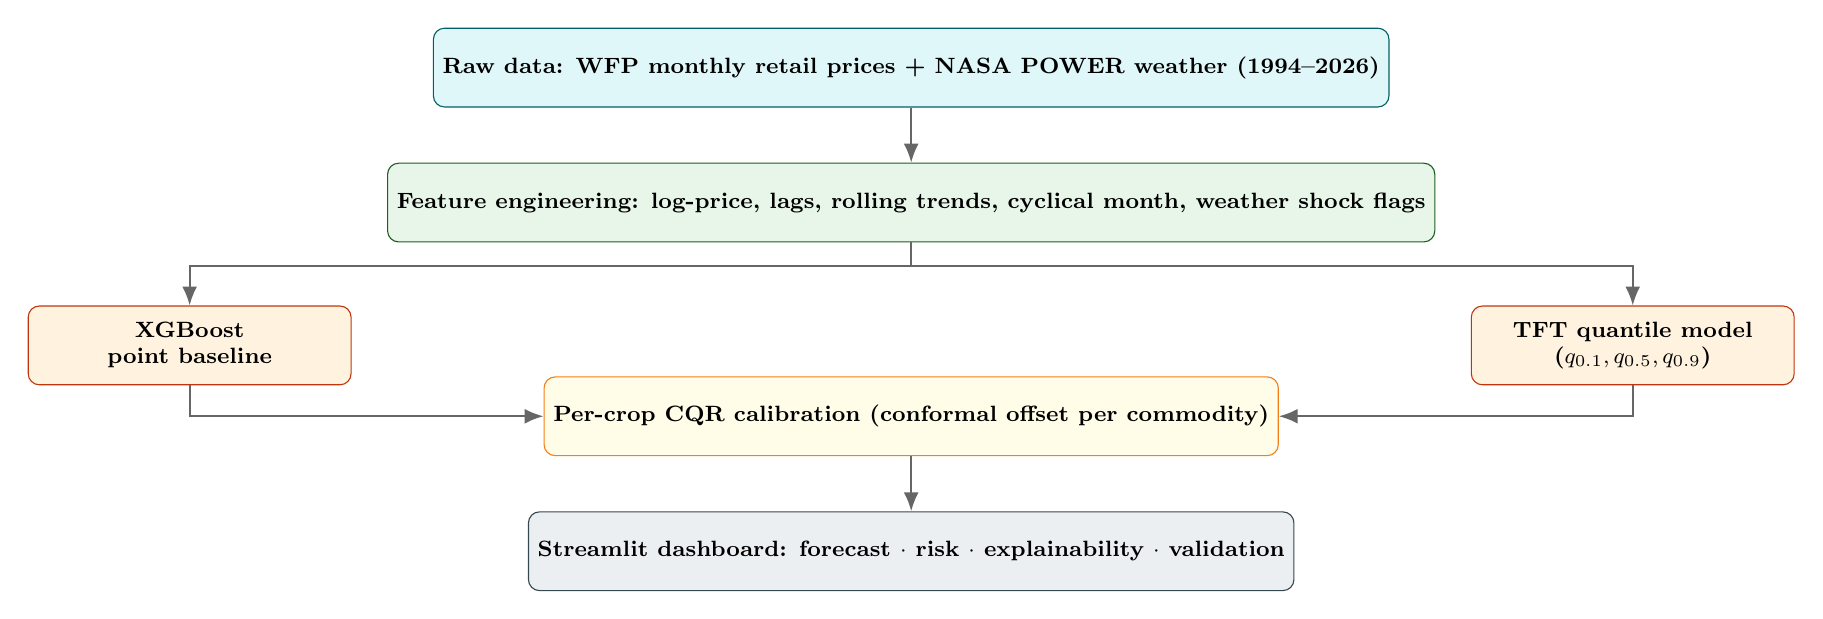
\begin{tikzpicture}[
    node distance=7mm,
    dnode/.style={draw=cdataborder, fill=cdata, rounded corners=4pt, align=center,
                  minimum width=9cm, minimum height=10mm, font=\footnotesize\bfseries},
    fnode/.style={draw=cfeatborder, fill=cfeat, rounded corners=4pt, align=center,
                  minimum width=9cm, minimum height=10mm, font=\footnotesize\bfseries},
    mnode/.style={draw=cmodelborder, fill=cmodel, rounded corners=4pt, align=center,
                  minimum width=4.1cm, minimum height=10mm, font=\footnotesize\bfseries},
    cnode/.style={draw=ccalibborder, fill=ccalib, rounded corners=4pt, align=center,
                  minimum width=9cm, minimum height=10mm, font=\footnotesize\bfseries},
    unode/.style={draw=cdeployborder, fill=cdeploy, rounded corners=4pt, align=center,
                  minimum width=9cm, minimum height=10mm, font=\footnotesize\bfseries},
    arr/.style={-{Latex[length=2.4mm,width=1.9mm]}, thick, draw=black!60}
]
\node[dnode] (raw) {Raw data: WFP monthly retail prices + NASA POWER weather (1994--2026)};
\node[fnode, below=of raw] (feat) {Feature engineering: log-price, lags, rolling trends, cyclical month, weather shock flags};
\node[mnode, below left=8mm and 4.5mm of feat] (xgb) {XGBoost\\point baseline};
\node[mnode, below right=8mm and 4.5mm of feat] (tft) {TFT quantile model\\($q_{0.1}, q_{0.5}, q_{0.9}$)};
\node[cnode, below=17mm of feat] (cal) {Per-crop CQR calibration (conformal offset per commodity)};
\node[unode, below=of cal] (dash) {Streamlit dashboard: forecast $\cdot$ risk $\cdot$ explainability $\cdot$ validation};
\draw[arr] (raw) -- (feat);
\draw[arr] (feat.south) -- ++(0,-3mm) -| (xgb.north);
\draw[arr] (feat.south) -- ++(0,-3mm) -| (tft.north);
\draw[arr] (xgb.south) |- (cal.west);
\draw[arr] (tft.south) |- (cal.east);
\draw[arr] (cal) -- (dash);
\end{tikzpicture}
}
\caption{Conceptual pipeline for the proposed crop price forecasting system.}
\label{fig:ch1_pipeline}
\end{figure}

\section{Contributions}

The main contributions of this work are summarized as follows.

\begin{itemize}
    \item \textbf{Reproducible multi-series pipeline:} A scripted data to model workflow
    for 53 markets and three crops, with all raw data, checkpoints, and calibration
    offsets version-controlled.

    \item \textbf{Calibrated probabilistic forecasting:} TFT-based quantile stack with
    per-crop CQR adjustment improving empirical coverage from 64.9 percent to 84.0 percent
    while simultaneously reducing prediction band width by 49 percent.

    \item \textbf{Leakage-controlled XGBoost fusion:} XGBoost predictions injected as
    known TFT covariates with a strict two-year temporal gap, achieving 50 percent MAE
    reduction and 60.8 percent MAPE reduction over TFT-Base.

    \item \textbf{Statistically validated interpretability:} Bootstrap analysis of Variable
    Selection Network (VSN) encoder weights (1000 resamples, Kendall $\tau = 0.942$)
    confirms stable feature attribution across market cohorts.

    \item \textbf{Unified decision interface:} Streamlit dashboard combining forecast
    trajectories, calibrated uncertainty, risk classification, VSN weights, and temporal
    attention in one reproducible workflow.
\end{itemize}

\section{Objective}

The primary objective is to develop a multi-series monthly price forecasting system for
Indian crop markets that delivers accurate point estimates, calibrated prediction intervals,
and interpretable feature attribution simultaneously. The system must be deployable through
an interactive dashboard usable by procurement planners and analysts without requiring
technical expertise in machine learning.

Table~\ref{tab:ch1_results} summarizes the headline test metrics achieved.

\begin{table}[H]
\centering
\caption{Headline test metrics on the 2023 test window (792 observations)}
\label{tab:ch1_results}
\small
\begin{tabularx}{\textwidth}{X
  >{\centering\arraybackslash}p{0.13\textwidth}
  >{\centering\arraybackslash}p{0.13\textwidth}
  >{\centering\arraybackslash}p{0.14\textwidth}
  >{\centering\arraybackslash}p{0.13\textwidth}}
\toprule
\textbf{Model Variant} & \textbf{MAE (Rs/kg)} & \textbf{MAPE (\%)} & \textbf{Coverage (\%)} & \textbf{Band Width} \\
\midrule
XGBoost baseline          & 1.58  & 2.8  & N/A  & N/A   \\
TFT-Base                  & 10.53 & 29.1 & 64.9 & 23.62 \\
TFT-EnsCQR                & 10.85 & 28.3 & 88.5 & 32.44 \\
TFT-Retrain21-CQR         & 9.91  & 29.2 & 87.6 & 34.78 \\
\textbf{TFT-XGBFusion-CQR} & \textbf{5.27} & \textbf{11.4} & \textbf{84.0} & \textbf{11.99} \\
\bottomrule
\end{tabularx}
\end{table}

%% =====================================================================
\chapter{Literature Survey}
%% =====================================================================

Agricultural crop price forecasting has a long history. Early statistical models gave way to
machine learning regressors, which are now being overtaken by deep sequence models. Despite
this progression, three gaps persist in the Indian crop price context: most studies optimise
point accuracy but not calibrated uncertainty; interpretation of model outputs is rarely
embedded in deployed tools; and direct comparison between probabilistic deep models and
strong baselines under a unified interface is uncommon.

\section{Classical Statistical Approaches}

Autoregressive Integrated Moving Average (ARIMA) and Seasonal ARIMA (SARIMA) models
(Box and Jenkins, 2015) are interpretable and handle linear trend and seasonality, but fail
under nonlinear shock dynamics common in Indian vegetable markets. Reported MAPE values
above 30 percent are common for volatile crops such as onions and tomatoes. Seasonal
decomposition methods face similar limitations when confronted with irregular supply shocks
that break the underlying periodicity assumptions.

\section{Machine Learning Approaches}

Gradient boosted trees, especially XGBoost, improve nonlinear fitting and are effective when
lag features are informative. XGBoost consistently outperforms ARIMA on monthly Indian crop
price data, but produces no calibrated uncertainty intervals. Support vector regression and
random forest models have also been applied, with comparable point accuracy but the same
absence of probabilistic output.

Manogna et al.\ (2025) demonstrated RNN, LSTM, and GRU models alongside XGBoost on a
large multi-crop, multi-market daily dataset, reporting onion MAPE of 14.59 percent for RNN
and 21.42 percent for XGBoost. These are point forecasts only and provide no uncertainty
quantification.

\section{Deep Learning Approaches}

LSTM and GRU models improve trend capture and allow multi-step forecasting. Transformer
variants improve horizon-level representation learning. The Temporal Fusion Transformer
(Lim et al., 2021) uniquely combines Variable Selection Networks (VSN), interpretable
multi-head attention, and quantile output heads in a single architecture. Unlike prior
approaches, TFT handles static metadata, known future covariates, and unknown historical
inputs in separate processing streams, making it well suited to market-level panel data
with exogenous weather variables.

Nayak et al.\ (2024) applied NBEATSX and XGBoost to weekly tomato, onion, and potato
crop prices, reporting an onion NBEATSX sMAPE of 11.25 percent. This approach, while
effective for weekly data, does not provide calibrated uncertainty or interpretable feature
attribution.

\section{Conformal Calibration}

Romano et al.\ (2019) proposed Conformalized Quantile Regression (CQR) as a
distribution-free post hoc method for constructing valid prediction intervals. It adjusts
pre-trained quantile outputs using a calibration set without retraining the underlying model.
The theoretical guarantee is marginal coverage: the true value falls within the adjusted
interval at least $(1-\alpha)$ fraction of the time under exchangeability. CQR is
particularly useful because it is model-agnostic and computationally lightweight.

\section{Gap in Existing Work}

From the above discussion, four consistent gaps motivate the present work.

\begin{itemize}
    \item Point accuracy is optimised but calibrated uncertainty is not evaluated.
    \item Strong baselines and probabilistic models are not compared under a unified
    interface.
    \item Coverage-oriented evaluation is under-reported in Indian crop price literature.
    \item Interpretability is rarely operationalised in deployed decision-support dashboards.
\end{itemize}

\section{Proposed Direction}

In contrast to prior work, this report addresses these gaps by combining probabilistic
forecasting (TFT) with a strong point baseline (XGBoost), injecting XGBoost predictions
as a feature to improve TFT accuracy, applying per-crop CQR calibration for reliable
intervals, and operationalising interpretability through a deployed dashboard.
This combination has not been demonstrated for Indian monthly crop price data at this scale.

\section{Literature Review Summary}

Table~\ref{tab:ch2_related} summarizes the representative studies and compares them with
the proposed approach.

\begin{table}[H]
\centering
\caption{Representative related studies and methodological comparison}
\label{tab:ch2_related}
\footnotesize
\setlength{\tabcolsep}{3pt}
\renewcommand{\arraystretch}{1.1}
\begin{tabular}{@{}p{0.19\textwidth}p{0.17\textwidth}p{0.17\textwidth}p{0.18\textwidth}p{0.23\textwidth}@{}}
\toprule
\textbf{Study} & \textbf{Data} & \textbf{Model} & \textbf{Best reported} & \textbf{Limitations} \\
\midrule
Nayak et al.\ (2024)   & TOP crops, weekly  & NBEATSX, XGBoost      & Onion sMAPE 11.25\%      & No uncertainty; no dashboard \\
Manogna et al.\ (2025) & 23 commodities, daily & RNN/LSTM, XGBoost  & Onion MAPE 14.59\%       & Point forecast only \\
Paul et al.\ (2022)    & Brinjal, 17 markets & GRNN, RF, SVR        & GRNN MAPE 3.68--17.86\% & No uncertainty; one crop \\
TFT tomato (2025)      & Tomato, 1 market   & TFT variants          & TFT sMAPE 22.03\%        & No fusion; no calibration \\
\textbf{This work}     & 3 crops, 53 markets & TFT + XGBoost + CQR  & Onion MAPE 9.1\%         & Monthly retail only \\
\bottomrule
\end{tabular}
\renewcommand{\arraystretch}{1.0}
\end{table}

%% =====================================================================
\chapter{Problem Statement}
%% =====================================================================

Crop price forecasting for Indian markets requires handling multiple sources of
non-stationarity: seasonal cycles driven by monsoon patterns, structural shocks from export
restrictions and supply chain disruptions, and cross-market correlations across geographically
dispersed trading hubs. Traditional approaches that model each crop and market in
isolation fail to leverage the shared temporal structure in the panel.

The specific challenge addressed in this work is: given monthly retail prices for a
market-crop pair and a set of exogenous features, forecast the next $H$ months with
(a) a central forecast (the 50th percentile, or median, $q_{0.5}$), (b) a calibrated
prediction interval defined by the 10th percentile ($q_{0.1}$, the low estimate) and the
90th percentile ($q_{0.9}$, the high estimate), and (c) interpretable feature importance
weights. The 10th and 90th percentile bounds together form a central 80 percent prediction
interval: in a well-calibrated model, the actual price should fall within this band
80 percent of the time. The test window covers 2023 onward, which includes the tomato price
spike and post-COVID price normalisation, both of which are out-of-distribution events
relative to the training period.

Formally, for a market-crop series with log-price $y_t$ at month $t$:
\[
\hat{y}_{t+h}^{(q)} = F_q\!\left(y_{t-L+1:t},\; z_{t-L+1:t},\; k_{t+1:t+H},\; s\right),
\quad h=1,\ldots,H,\quad q \in \{0.1,\,0.5,\,0.9\}.
\]
Here $L=24$ is the encoder look-back window, $H=6$ is the prediction horizon, $z$ are
observed historical covariates, $k$ are known future covariates (calendar and seasonal flags),
and $s$ is the static market-crop identity. Training uses pinball (quantile) loss:
\[
\mathcal{L}_q(y,\hat{y})=
\begin{cases}
q\,(y-\hat{y}), & y \ge \hat{y}, \\[2pt]
(1-q)\,(\hat{y}-y), & y < \hat{y}.
\end{cases}
\]
Empirical coverage over $N$ test points is:
\[
\text{Coverage}=\frac{1}{N}\sum_{i=1}^{N}\mathbf{1}\!\left[\hat{y}_{i}^{(0.1)}\le y_i \le \hat{y}_{i}^{(0.9)}\right].
\]
The target is to minimise MAE and MAPE while maintaining empirical coverage above 80 percent
at practically narrow interval widths. No prior work on Indian crop prices has simultaneously
optimised all three objectives within a single deployed system.

%% =====================================================================
\chapter{Dataset}
%% =====================================================================

\section{Data Sources}

Two external sources are used. The World Food Programme (WFP) provides monthly retail crop
price records for India under a CC~BY license, covering January 1994 to February 2026 ---
over 30 years spanning multiple drought events, flood years, and the COVID-19 disruption.
NASA POWER (Prediction Of Worldwide Energy Resources) provides satellite-derived monthly
weather variables --- temperature, rainfall, and humidity --- aligned to each market's GPS
coordinates through its public API.

For each of the 53 markets in the modeling dataset, a market-to-GPS lookup was constructed.
For each (market, year, month) combination, the NASA POWER monthly point API was queried
for three variables: T2M (mean temperature at 2 m height), PRECTOTCORR (total monthly
precipitation), and RH2M (mean relative humidity at 2 m height). Responses were cached
locally to avoid repeated API calls.

\begin{table}[H]
\centering
\caption{Data lineage from raw source to modeling dataset}
\label{tab:ch4_data_audit}
\small
\begin{tabularx}{\textwidth}{L{0.26\textwidth}L{0.20\textwidth}L{0.20\textwidth}X}
\toprule
\textbf{Stage} & \textbf{Rows} & \textbf{Series/Markets} & \textbf{Notes} \\
\midrule
Raw WFP file & 145,124 & 170 markets, 41 commodities & 1994-01 to 2026-02 \\
Filtered prices & 18,415 & 123 series, 53 markets & Retail-only, series-length filter \\
Master dataset & 16,939 & 123 series, 53 markets & After weather merge and lag warm-up removal \\
\bottomrule
\end{tabularx}
\end{table}

Three crops were chosen to represent distinct volatility regimes. Volatility is measured
here by the Coefficient of Variation (CV), which is the ratio of the standard deviation to
the mean expressed as a percentage. A high CV means prices fluctuate widely around the
average. Onions have a CV of about 60 percent (highest volatility, monsoon driven supply
shocks). Tomatoes have a CV of about 90 percent (highly event sensitive, with the 2023
price spike falling in the test window). Rice has a CV of about 20 percent (stable staple
with government procurement support, which tests whether the model can also produce tight
intervals for low-volatility series).

\section{Feature Engineering}

Six filtering steps produce the modeling dataset: remove aggregate rows; keep retail records
only; retain target crops in kg units; normalise duplicate market labels; remove
duplicate date-market keys; retain series with at least 60 monthly observations. Short gaps
of three months or fewer are forward-filled; series with gaps longer than six months are
dropped. A contiguous monthly integer index is assigned as
$\text{time\_idx} = 12\,(\text{year}-1994) + (\text{month}-1)$.

\begin{table}[H]
\centering
\caption{Feature groups in the master dataset (26 columns total)}
\label{tab:ch4_features}
\small
\setlength{\tabcolsep}{3pt}
\begin{tabularx}{\textwidth}{@{}L{0.22\textwidth}L{0.32\textwidth}X@{}}
\toprule
\textbf{Group} & \textbf{Columns} & \textbf{Purpose} \\
\midrule
Identifiers & series\_id, commodity, market, admin1, date, price & Series grouping and context \\
Temporal & time\_idx, year, month, season, month\_sin, month\_cos, covid\_lockdown & Calendar structure and known future covariates \\
Target and trend & log\_price, price\_lag\_1m, price\_lag\_12m, rolling\_3m, rolling\_6m, yoy\_change & Momentum, annual memory, trend persistence \\
Weather & temperature\_mean, rainfall\_monthly, humidity\_mean & Exogenous environmental signals \\
Shock flags & rain\_deficit, rain\_excess, heat\_stress, cold\_stress & Binary indicators for adverse climate events \\
\bottomrule
\end{tabularx}
\end{table}

\section{Train-Test Split}

A strict chronological split is used throughout to prevent future data from leaking into
the training set. If rows were split randomly, months from 2023 could appear in the training
set, allowing the model to observe future prices during training and inflate test accuracy.
Instead, the split follows calendar order as shown in Table~\ref{tab:ch4_splits}.

\begin{table}[H]
\centering
\caption{Temporal split for each model family}
\label{tab:ch4_splits}
\small
\begin{tabularx}{\textwidth}{L{0.28\textwidth}L{0.24\textwidth}L{0.20\textwidth}X}
\toprule
\textbf{Family} & \textbf{Train} & \textbf{Validation} & \textbf{Test} \\
\midrule
TFT-Base & $\le$ 2020-12-31 (13,227 rows) & 2021--2022 (2,920 rows) & 2023+ (792 rows) \\
TFT-XGBFusion / Retrain21 & $\le$ 2021-12-31 (14,686 rows) & 2022 (1,461 rows) & 2023+ (792 rows) \\
\bottomrule
\end{tabularx}
\end{table}

The XGBoost model used as the fusion covariate source is trained only on data up to
2019-12-31, providing a two-year gap relative to TFT training. All evaluation is performed
on the 2023 held-out window (792 rows) across 123 market-crop series.

\section{Dataset Statistics}

\begin{table}[H]
\centering
\caption{Crop coverage in the master dataset}
\label{tab:ch4_commodity}
\small
\begin{tabularx}{\textwidth}{L{0.20\textwidth}
    >{\centering\arraybackslash}p{0.10\textwidth}
    >{\centering\arraybackslash}p{0.10\textwidth}
    >{\centering\arraybackslash}p{0.12\textwidth}X}
\toprule
\textbf{Crop} & \textbf{Rows} & \textbf{Series} & \textbf{Markets} & \textbf{Role} \\
\midrule
Onions    & 5,003 & 38 & 38 & Highest volatility; monsoon driven supply shocks \\
Tomatoes  & 5,245 & 45 & 45 & Event sensitive; 2023 price spike in test window \\
Rice      & 6,691 & 40 & 40 & Stable staple; tests interval tightness \\
\bottomrule
\end{tabularx}
\end{table}

%% =====================================================================
\chapter{Methodology}
%% =====================================================================

\section{Overall Pipeline}

The system is built around five pipeline stages: data build, model training, prediction and
calibration, evaluation and explainability, and deployment. Figure~\ref{fig:ch5_pipeline}
maps execution to these stages.

\begin{figure}[H]
\centering
\resizebox{0.90\textwidth}{!}{%
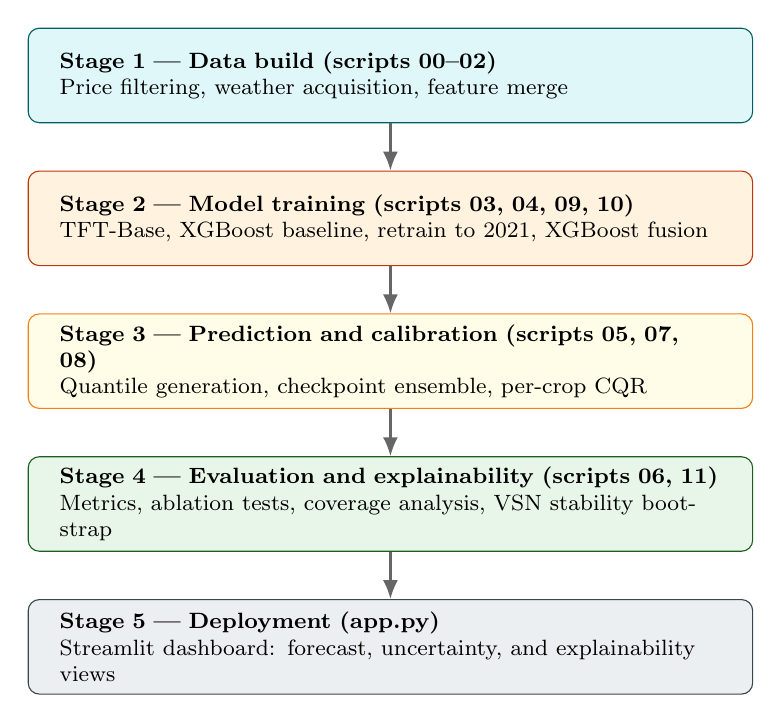
\begin{tikzpicture}[
    node distance=6mm,
    s1/.style={draw=cdataborder, fill=cdata, rounded corners=4pt, align=left,
               minimum width=9.2cm, minimum height=12mm, text width=8.4cm, font=\footnotesize},
    s2/.style={draw=cmodelborder, fill=cmodel, rounded corners=4pt, align=left,
               minimum width=9.2cm, minimum height=12mm, text width=8.4cm, font=\footnotesize},
    s3/.style={draw=ccalibborder, fill=ccalib, rounded corners=4pt, align=left,
               minimum width=9.2cm, minimum height=12mm, text width=8.4cm, font=\footnotesize},
    s4/.style={draw=cfeatborder, fill=cfeat, rounded corners=4pt, align=left,
               minimum width=9.2cm, minimum height=12mm, text width=8.4cm, font=\footnotesize},
    s5/.style={draw=cdeployborder, fill=cdeploy, rounded corners=4pt, align=left,
               minimum width=9.2cm, minimum height=12mm, text width=8.4cm, font=\footnotesize},
    arr/.style={-{Latex[length=2.4mm,width=1.9mm]}, thick, draw=black!60}
]
\node[s1] (s0) {\textbf{Stage 1 --- Data build (scripts 00--02)}\\Price filtering, weather acquisition, feature merge};
\node[s2, below=of s0] (s1) {\textbf{Stage 2 --- Model training (scripts 03, 04, 09, 10)}\\TFT-Base, XGBoost baseline, retrain to 2021, XGBoost fusion};
\node[s3, below=of s1] (s2) {\textbf{Stage 3 --- Prediction and calibration (scripts 05, 07, 08)}\\Quantile generation, checkpoint ensemble, per-crop CQR};
\node[s4, below=of s2] (s3) {\textbf{Stage 4 --- Evaluation and explainability (scripts 06, 11)}\\Metrics, ablation tests, coverage analysis, VSN stability bootstrap};
\node[s5, below=of s3] (s4) {\textbf{Stage 5 --- Deployment (app.py)}\\Streamlit dashboard: forecast, uncertainty, and explainability views};
\draw[arr] (s0) -- (s1);
\draw[arr] (s1) -- (s2);
\draw[arr] (s2) -- (s3);
\draw[arr] (s3) -- (s4);
\end{tikzpicture}
}
\caption{Operational pipeline from data processing to dashboard deployment.}
\label{fig:ch5_pipeline}
\end{figure}

\section{XGBoost Baseline}

An XGBoost gradient boosted tree regressor operates in log-price space:
\[
\hat{y}_t = \sum_{m=1}^{M} \nu\, f_m(\mathbf{u}_t),
\]
where each $f_m$ is a regression tree, $\nu$ is the learning rate, and $\mathbf{u}_t$
includes the one-month lag, twelve-month lag, three-month and six-month rolling means,
year on year change, and weather variables. The model is trained on data up to 2019-12-31
to maintain a two-year gap from the TFT training window. XGBoost achieves the lowest
point forecast MAE (1.58 Rs per kg) because it directly minimises squared error over
high-information lag features. It provides no calibrated uncertainty interval.

\section{Temporal Fusion Transformer}

The Temporal Fusion Transformer (Lim et al., 2021) handles multi-horizon quantile
forecasting with built-in interpretability. Figure~\ref{fig:ch5_tft} shows its structure:
three input streams through Variable Selection Networks (VSN), an LSTM encoder-decoder with
static context injection, interpretable multi-head attention, and quantile output heads.

\begin{figure}[H]
\centering
\resizebox{0.96\textwidth}{!}{%
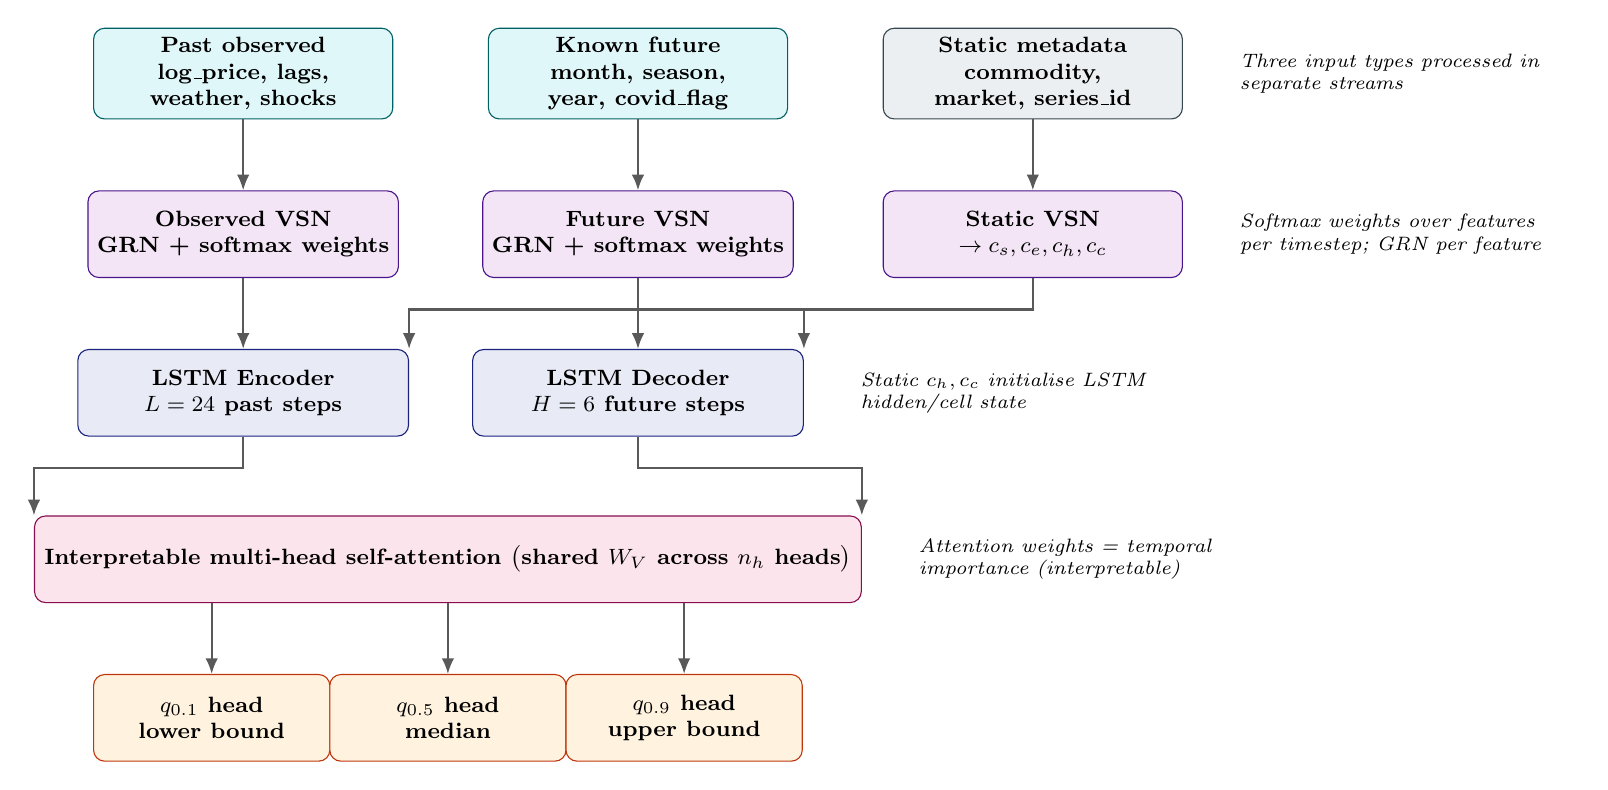
\begin{tikzpicture}[
    node distance=8mm and 15mm,
    inp/.style={draw=cdataborder, fill=cdata, rounded corners=4pt, align=center,
                minimum width=3.8cm, minimum height=11mm, font=\footnotesize\bfseries},
    vsn/.style={draw=cvsnborder, fill=cvsn, rounded corners=4pt, align=center,
                minimum width=3.8cm, minimum height=11mm, font=\footnotesize\bfseries},
    lstm/.style={draw=clstmborder, fill=clstm, rounded corners=4pt, align=center,
                 minimum width=4.2cm, minimum height=11mm, font=\footnotesize\bfseries},
    stat/.style={draw=cdeployborder, fill=cdeploy, rounded corners=4pt, align=center,
                 minimum width=3.8cm, minimum height=11mm, font=\footnotesize\bfseries},
    attn/.style={draw=cattnborder, fill=cattn, rounded corners=4pt, align=center,
                 minimum width=10.5cm, minimum height=11mm, font=\footnotesize\bfseries},
    qout/.style={draw=cmodelborder, fill=cmodel, rounded corners=4pt, align=center,
                minimum width=3.0cm, minimum height=11mm, font=\footnotesize\bfseries},
    ann/.style={font=\scriptsize\itshape, align=left, text width=4.2cm},
    arr/.style={-{Latex[length=2mm,width=1.6mm]}, thick, draw=black!65}
]
\node[inp] (pi) {Past observed\\log\_price, lags,\\weather, shocks};
\node[inp, right=12mm of pi] (fi) {Known future\\month, season,\\year, covid\_flag};
\node[stat, right=12mm of fi] (si) {Static metadata\\commodity,\\market, series\_id};

\node[vsn, below=9mm of pi] (pv) {Observed VSN\\GRN + softmax weights};
\node[vsn, below=9mm of fi] (fv) {Future VSN\\GRN + softmax weights};
\node[vsn, below=9mm of si] (sv) {Static VSN\\$\to c_s, c_e, c_h, c_c$};

\node[lstm, below=9mm of pv] (le) {LSTM Encoder\\$L = 24$ past steps};
\node[lstm, below=9mm of fv] (ld) {LSTM Decoder\\$H = 6$ future steps};

\node[attn, below=10mm of le, xshift=2.6cm] (att) {Interpretable multi-head self-attention $\bigl($shared $W_V$ across $n_h$ heads$\bigr)$};

\node[qout, below=9mm of att, xshift=-3.0cm] (q1) {$q_{0.1}$ head\\lower bound};
\node[qout, below=9mm of att] (q5) {$q_{0.5}$ head\\median};
\node[qout, below=9mm of att, xshift=3.0cm] (q9) {$q_{0.9}$ head\\upper bound};

\node[ann, right=6mm of si] {Three input types processed in separate streams};
\node[ann, right=6mm of sv] {Softmax weights over features per timestep; GRN per feature};
\node[ann, right=6mm of ld] {Static $c_h, c_c$ initialise LSTM hidden/cell state};
\node[ann, right=6mm of att] {Attention weights = temporal importance (interpretable)};

\draw[arr] (pi) -- (pv);
\draw[arr] (fi) -- (fv);
\draw[arr] (si) -- (sv);
\draw[arr] (pv) -- (le);
\draw[arr] (fv) -- (ld);
\draw[arr] (sv.south) -- ++(0,-4mm) -| (le.north east);
\draw[arr] (sv.south) -- ++(0,-4mm) -| (ld.north east);
\draw[arr] (le.south) -- ++(0,-4mm) -| (att.north west);
\draw[arr] (ld.south) -- ++(0,-4mm) -| (att.north east);
\draw[arr] ($(att.south)+(-3.0cm,0)$) -- (q1.north);
\draw[arr] (att.south) -- (q5.north);
\draw[arr] ($(att.south)+(3.0cm,0)$) -- (q9.north);
\end{tikzpicture}
}
\caption{TFT architecture: three input streams through VSN layers, LSTM encoder-decoder
with static context injection, interpretable multi-head attention, and three quantile output heads.}
\label{fig:ch5_tft}
\end{figure}

\subsection{Variable Selection Networks}

Variable Selection Networks (VSN) learn per-timestep softmax weights over all features via
Gated Residual Networks (GRN). For each timestep, a GRN is applied to each input feature
independently, and a second GRN produces the softmax weights over all features. The output
is a weighted combination of transformed features. These weights are the primary
interpretability output of TFT: they indicate which features the model relies on most at
each point in the input sequence.

\subsection{LSTM Encoder-Decoder}

The LSTM encoder reads 24 past observations and produces a sequence of hidden states.
The LSTM decoder processes 6 future steps. Static embeddings derived from the Static VSN
initialise the LSTM hidden and cell states, allowing the model to condition forecasts on the
identity of the market and crop. A gating mechanism controls how much of each hidden state
passes to the attention layer.

\subsection{Interpretable Multi-Head Attention and Quantile Heads}

The attention layer uses a shared value matrix $W_V$ across all heads. This makes the
aggregated attention weights interpretable as position-level temporal importance: high
attention on month $t-k$ means the model found historical context $k$ steps ago informative
for the current forecast. Three quantile output heads independently produce $q_{0.1}$,
$q_{0.5}$, and $q_{0.9}$ for each future horizon, trained jointly with pinball loss.

The 10th percentile head ($q_{0.1}$) gives the low price estimate, the 50th percentile head
($q_{0.5}$) gives the median or central prediction, and the 90th percentile head ($q_{0.9}$)
gives the high price estimate. Together these form a central 80 percent prediction interval.

\begin{table}[H]
\centering
\caption{TFT training configuration (consistent across all model families)}
\label{tab:ch5_tft_config}
\small
\begin{tabularx}{\textwidth}{L{0.36\textwidth}L{0.18\textwidth}X}
\toprule
\textbf{Parameter} & \textbf{Value} & \textbf{Rationale} \\
\midrule
hidden\_size            & 32       & Compact for monthly panel; prevents overfitting \\
attention\_head\_size   & 2        & Balance between diversity and stability \\
lstm\_layers            & 1        & Limits overfitting in small to medium panel \\
dropout                 & 0.2      & Cross-series regularisation \\
quantiles               & 0.1, 0.5, 0.9 & Direct probabilistic forecasting \\
max\_encoder\_length    & 24 months & Annual cycle plus trend memory \\
max\_prediction\_length & 6 months  & Short to medium planning horizon \\
learning\_rate          & 0.03      & Stable convergence under Ranger optimizer \\
\bottomrule
\end{tabularx}
\end{table}

\section{XGBoost-TFT Feature Fusion}

In TFT-XGBFusion, the log-price prediction from the pre-2020 XGBoost model is injected as a
known covariate (\texttt{xgb\_log\_pred}) at every future timestep. This design exploits
XGBoost's local lag accuracy as a structured prior for TFT while preserving a strict
two-year gap: the XGBoost model is trained on data up to 2019-12-31, and TFT training uses
data up to 2021-12-31.

This approach is fundamentally different from model stacking (Wolpert, 1992), in which two
models predict independently and their outputs are blended afterward. Here TFT receives the
XGBoost prediction as a feature and decides through its VSN how much weight to assign to it
at each timestep. For a stable rice market the XGBoost signal is likely accurate and TFT
can assign high weight to it. During a tomato spike, if XGBoost underestimates because tree
models do not extrapolate to previously unseen price levels, TFT can downweight that signal
and rely on its own sequential reasoning.

The result is a 50 percent MAE reduction (from 10.53 Rs per kg to 5.27 Rs per kg) and a
60.8 percent MAPE reduction (from 29.1 percent to 11.4 percent) over TFT-Base, while also
reducing the calibrated interval width by 49 percent.

\section{Conformal Quantile Regression Calibration}

TFT-Base achieves only 64.9 percent coverage on the test set, well below expectation for a
$q_{0.1}$--$q_{0.9}$ interval. CQR (Romano et al., 2019) corrects this without retraining.
For each calibration sample $i$:
\[
E_i = \max\!\left(q_{0.1,i}-y_i,\; y_i-q_{0.9,i}\right).
\]
For target miscoverage $\alpha=0.10$, the per-crop offset is:
\[
\hat{Q}_{\alpha} = \mathrm{Quantile}_{1-\alpha}\!\left(\{E_i\}_{i=1}^{n}\right).
\]
Calibrated bounds are then:
\[
\tilde{q}_{0.1}=q_{0.1}-\hat{Q}_{\alpha},
\qquad
\tilde{q}_{0.9}=q_{0.9}+\hat{Q}_{\alpha}.
\]
The median $q_{0.5}$ is unchanged. Calibration offsets are computed separately per crop,
allowing the system to account for the different tail behaviour of onions, tomatoes, and rice.
A global offset would over-widen the rice interval and under-widen the tomato interval.

\section{Evaluation Metrics}

Point accuracy is measured by MAE (Rs per kg), RMSE (Rs per kg), and MAPE (percent) in
original price scale after exponentiating log-space predictions. Interval quality is measured
by empirical coverage and mean band width. Statistical significance of improvements is
assessed using paired $t$-tests and Wilcoxon signed-rank tests, and effect size is reported
as Cohen's $d$. Interpretability stability is assessed through 1000-resample bootstrap of
VSN encoder weights with mean pairwise Kendall $\tau$.

%% =====================================================================
\chapter{Results and Analysis}
%% =====================================================================

\section{Model Comparison}

Table~\ref{tab:ch6_metrics} presents the full comparison of all model families on the 2023
test window. Two patterns stand out. First, XGBoost dominates on point accuracy, reaching
an MAE of 1.58 Rs per kg by directly minimising squared error over high-information lag
features. Second, TFT-Base's 64.9 percent coverage confirms that raw quantile training is
insufficient for reliable uncertainty bounds. CQR calibration is essential, not optional.

\begin{table}[H]
\centering
\caption{Test metrics (2023, 792 rows) across all model families}
\label{tab:ch6_metrics}
\small
\setlength{\tabcolsep}{3pt}
\begin{tabularx}{\textwidth}{@{}L{0.36\textwidth}
  >{\centering\arraybackslash}p{0.13\textwidth}
  >{\centering\arraybackslash}p{0.13\textwidth}
  >{\centering\arraybackslash}p{0.14\textwidth}
  >{\centering\arraybackslash}p{0.14\textwidth}@{}}
\toprule
\textbf{Model variant} & \textbf{MAE (Rs/kg)} & \textbf{MAPE (\%)} & \textbf{Coverage (\%)} & \textbf{Band width} \\
\midrule
XGBoost baseline           & 1.58  & 2.8  & N/A  & N/A   \\
TFT-Base                   & 10.53 & 29.1 & 64.9 & 23.62 \\
TFT-EnsCQR                 & 10.85 & 28.3 & 88.5 & 32.44 \\
TFT-Retrain21-CQR          & 9.91  & 29.2 & 87.6 & 34.78 \\
\textbf{TFT-XGBFusion-CQR} & \textbf{5.27} & \textbf{11.4} & \textbf{84.0} & \textbf{11.99} \\
\bottomrule
\end{tabularx}
\end{table}

\section{Ablation Study}

Relative to TFT-Base, TFT-XGBFusion-CQR achieves 60.8 percent MAPE reduction (29.1 to
11.4 percent) and 50.0 percent MAE reduction (10.53 Rs per kg to 5.27 Rs per kg). Coverage
improves by 19.1 percentage points while band width decreases by 49.2 percent. Critically,
TFT-EnsCQR reaches 88.5 percent coverage but at a width of 32.44 Rs per kg, nearly three
times wider than TFT-XGBFusion-CQR at 11.99 Rs per kg. Wider coverage alone is not a
better outcome; the fusion model achieves a superior accuracy-calibration balance.

Paired statistical tests confirm the improvement over TFT-Base:
$t = -22.34$, $p = 4.6 \times 10^{-86}$, Cohen's $d = -0.79$ (large effect), Wilcoxon
$p = 1.2 \times 10^{-95}$. The step from TFT-Base to TFT-Retrain21-CQR (adding only
extended cutoff) shows a smaller but significant contribution:
$t = -4.15$, $p = 3.6 \times 10^{-5}$, Cohen's $d = -0.15$.

\begin{figure}[H]
\centering
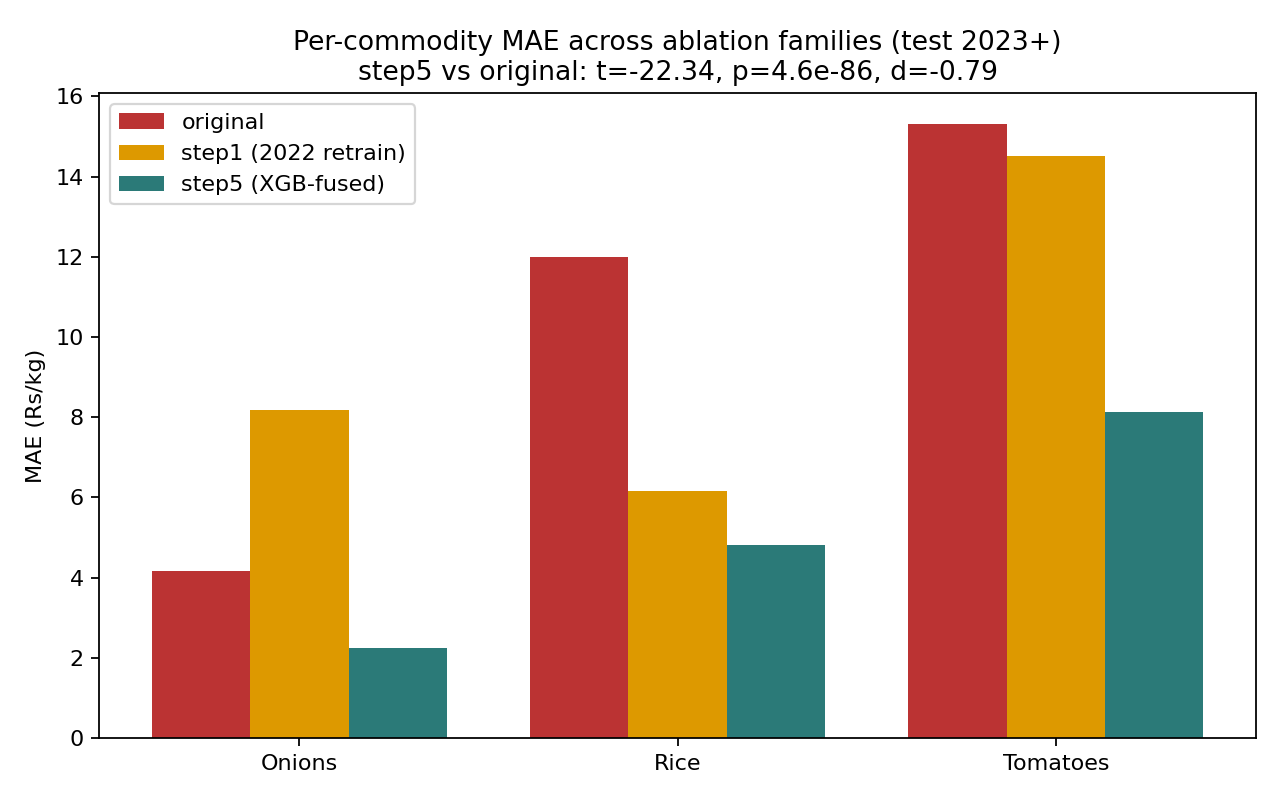
\includegraphics[width=0.85\textwidth]{figures/paper/fig_ablation_mae.png}
\caption{Per-crop MAE across TFT variants (2023 test period).
TFT-XGBFusion-CQR achieves the lowest MAE on all three crops.}
\label{fig:ch6_ablation}
\end{figure}

\begin{figure}[H]
\centering
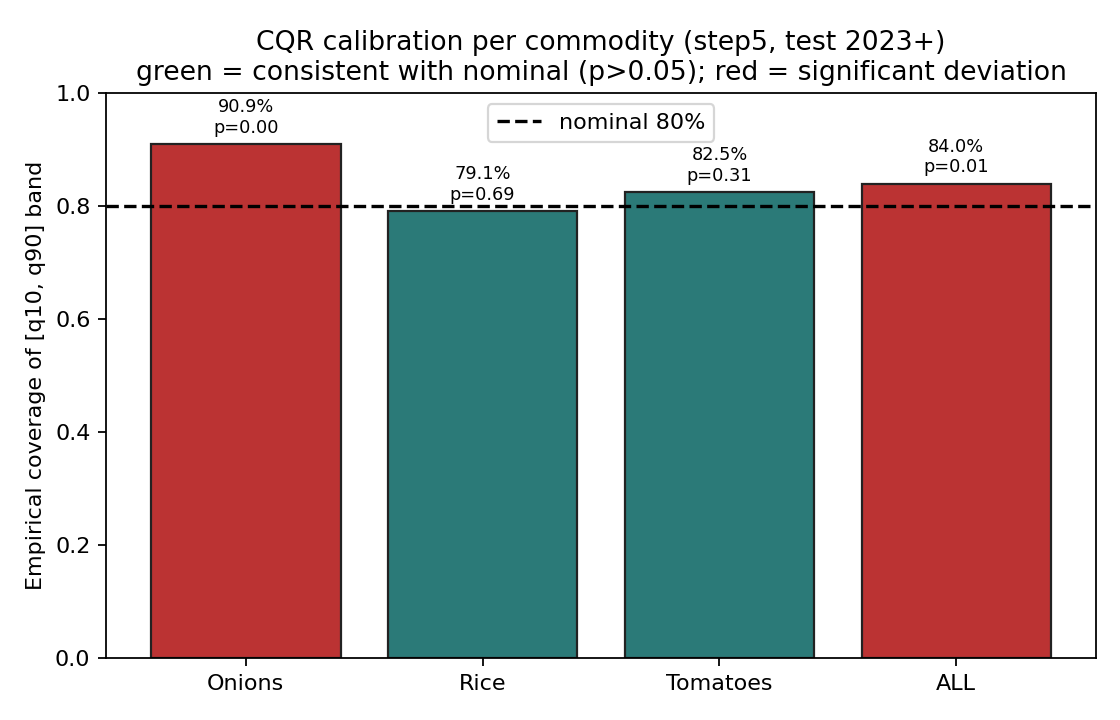
\includegraphics[width=0.85\textwidth]{figures/paper/fig_calibration_coverage.png}
\caption{Empirical coverage of the calibrated $q_{0.1}$--$q_{0.9}$ interval
(TFT-XGBFusion-CQR, 2023 test set). Dashed line shows the 80 percent nominal target.
Bars statistically consistent with the target ($p > 0.05$) are shown in green.}
\label{fig:ch6_coverage}
\end{figure}

\section{Variable Importance Stability}

Bootstrap analysis (1000 series-level resamples) of VSN encoder weights yields mean
pairwise Kendall $\tau = 0.942$ with a 95 percent confidence interval of [0.895, 0.990].
This indicates that the feature ranking is highly stable across different subsets of the
market-crop panel, which is a necessary condition for trusting VSN weights as interpretable
signals.

Top encoder features by mean importance: temperature\_mean (0.1432), rain\_excess (0.1427),
rain\_deficit (0.1402), humidity\_mean (0.0664), year (0.0600), covid\_lockdown (0.0587),
season (0.0419), log\_price (0.0405), rolling\_6m (0.0382), price\_lag\_12m (0.0381).
Weather variables dominate the top three, consistent with monsoon driven supply shocks being
the primary driver of price volatility in Indian vegetable markets.

\begin{figure}[H]
\centering
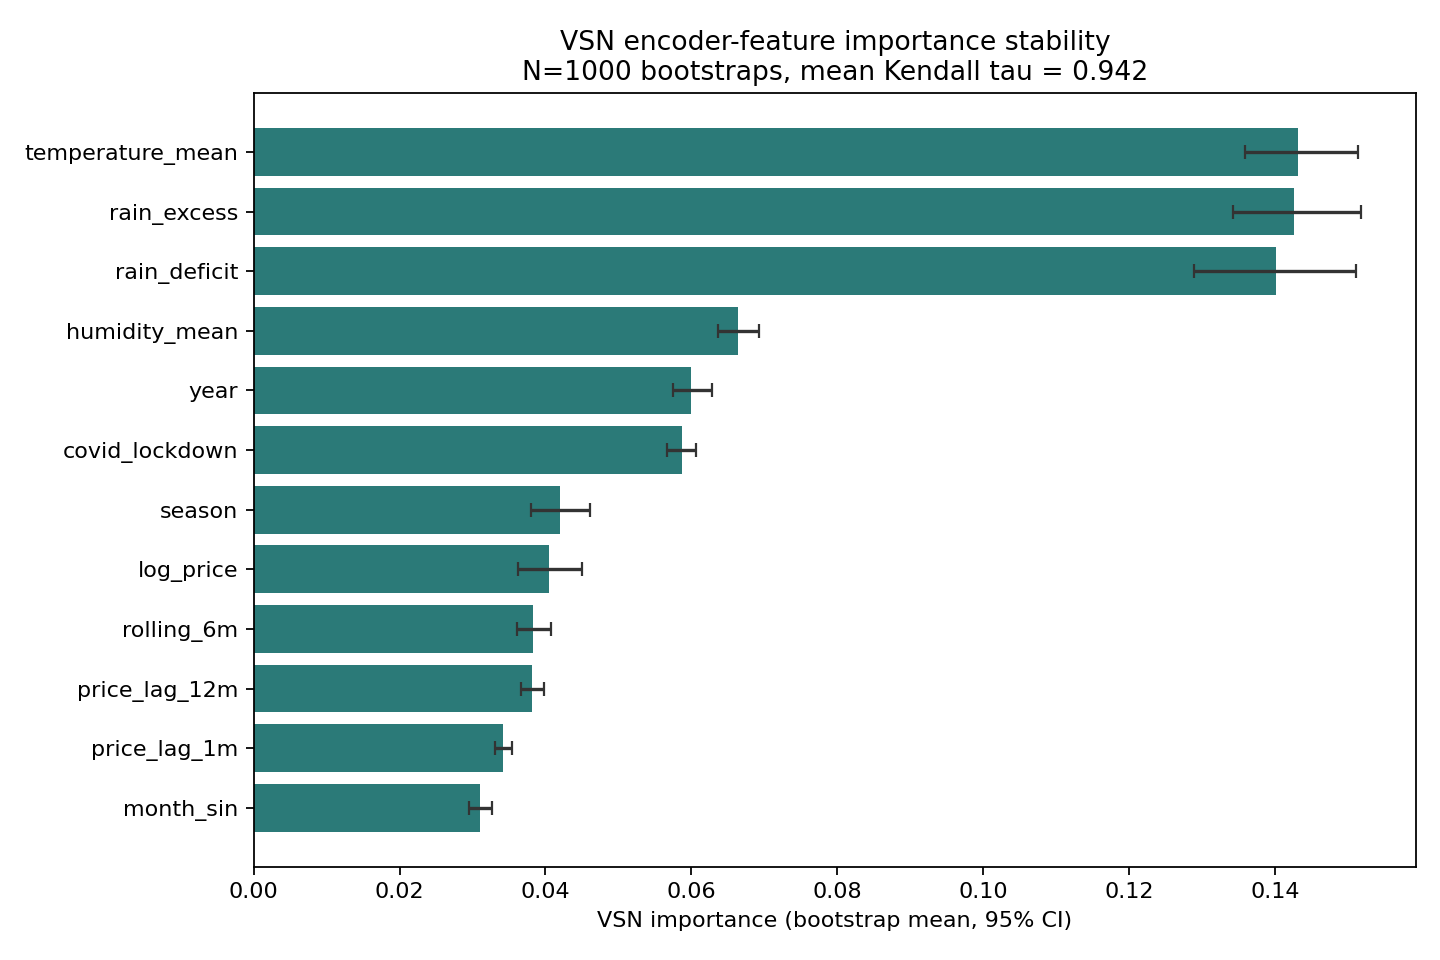
\includegraphics[width=0.85\textwidth]{figures/paper/fig_vsn_stability.png}
\caption{Bootstrap stability of TFT encoder VSN importances (1000 resamples). Kendall
$\tau = 0.942$ confirms stable feature ranking across market-crop series cohorts.}
\label{fig:ch6_vsn}
\end{figure}

\begin{figure}[H]
\centering
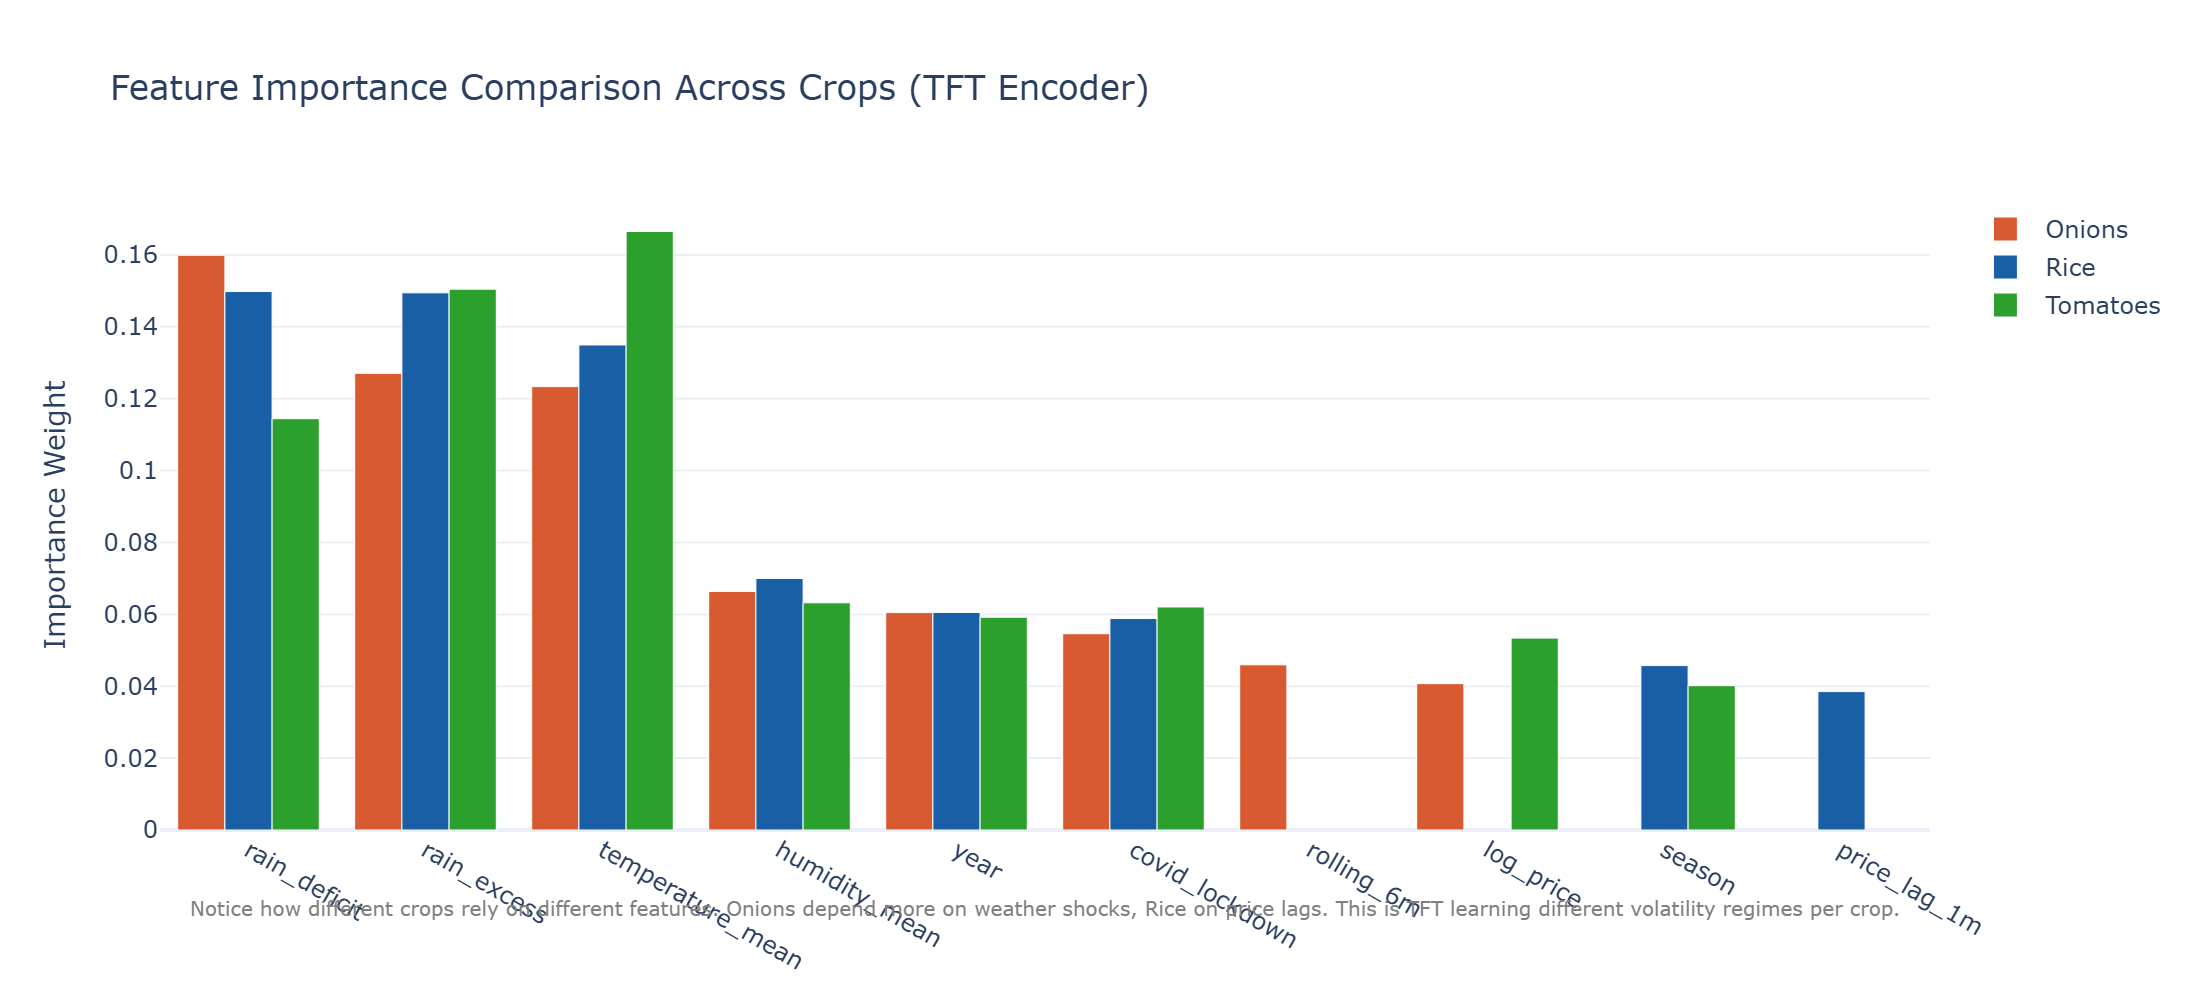
\includegraphics[width=0.85\textwidth]{figures/paper/variable_importance_comparison.png}
\caption{Comparison of encoder and decoder VSN feature importances. Weather related features
and price memory variables dominate consistently across both pathways.}
\label{fig:ch6_varimp}
\end{figure}

\section{Crop-wise Analysis}

\begin{table}[H]
\centering
\caption{Crop-wise test metrics for TFT-XGBFusion-CQR (2023 test set)}
\label{tab:ch6_commodity}
\small
\begin{tabularx}{\textwidth}{L{0.20\textwidth}
    >{\centering\arraybackslash}p{0.14\textwidth}
    >{\centering\arraybackslash}p{0.14\textwidth}
    >{\centering\arraybackslash}p{0.14\textwidth}X}
\toprule
\textbf{Crop} & \textbf{MAE (Rs/kg)} & \textbf{MAPE (\%)} & \textbf{Coverage (\%)} & \textbf{Observations} \\
\midrule
Onions   & 2.25 & 9.1  & 90.9 & Best accuracy; conservative interval \\
Tomatoes & 8.13 & 13.0 & 82.5 & Hardest series; 2023 spike in test window \\
Rice     & 4.81 & 11.7 & 79.1 & Stable regime; narrowest intervals \\
\midrule
\textbf{Overall} & \textbf{5.27} & \textbf{11.4} & \textbf{84.0} & n=792 observations \\
\bottomrule
\end{tabularx}
\end{table}

Figures~\ref{fig:ch6_qf_onions}--\ref{fig:ch6_qf_rice} show the calibrated TFT-XGBFusion-CQR prediction
range overlaid on actual prices for each crop in the 2023 test period. The shaded band
represents the central 80 percent prediction interval ($q_{0.1}^{\text{cal}}$ to
$q_{0.9}^{\text{cal}}$) and the solid line is the median prediction. The onion and rice
forecasts track actual prices closely. The tomato forecast correctly produces a wider band
during the mid-2023 price surge, reflecting higher prediction uncertainty for that crop.

\begin{figure}[H]
\centering
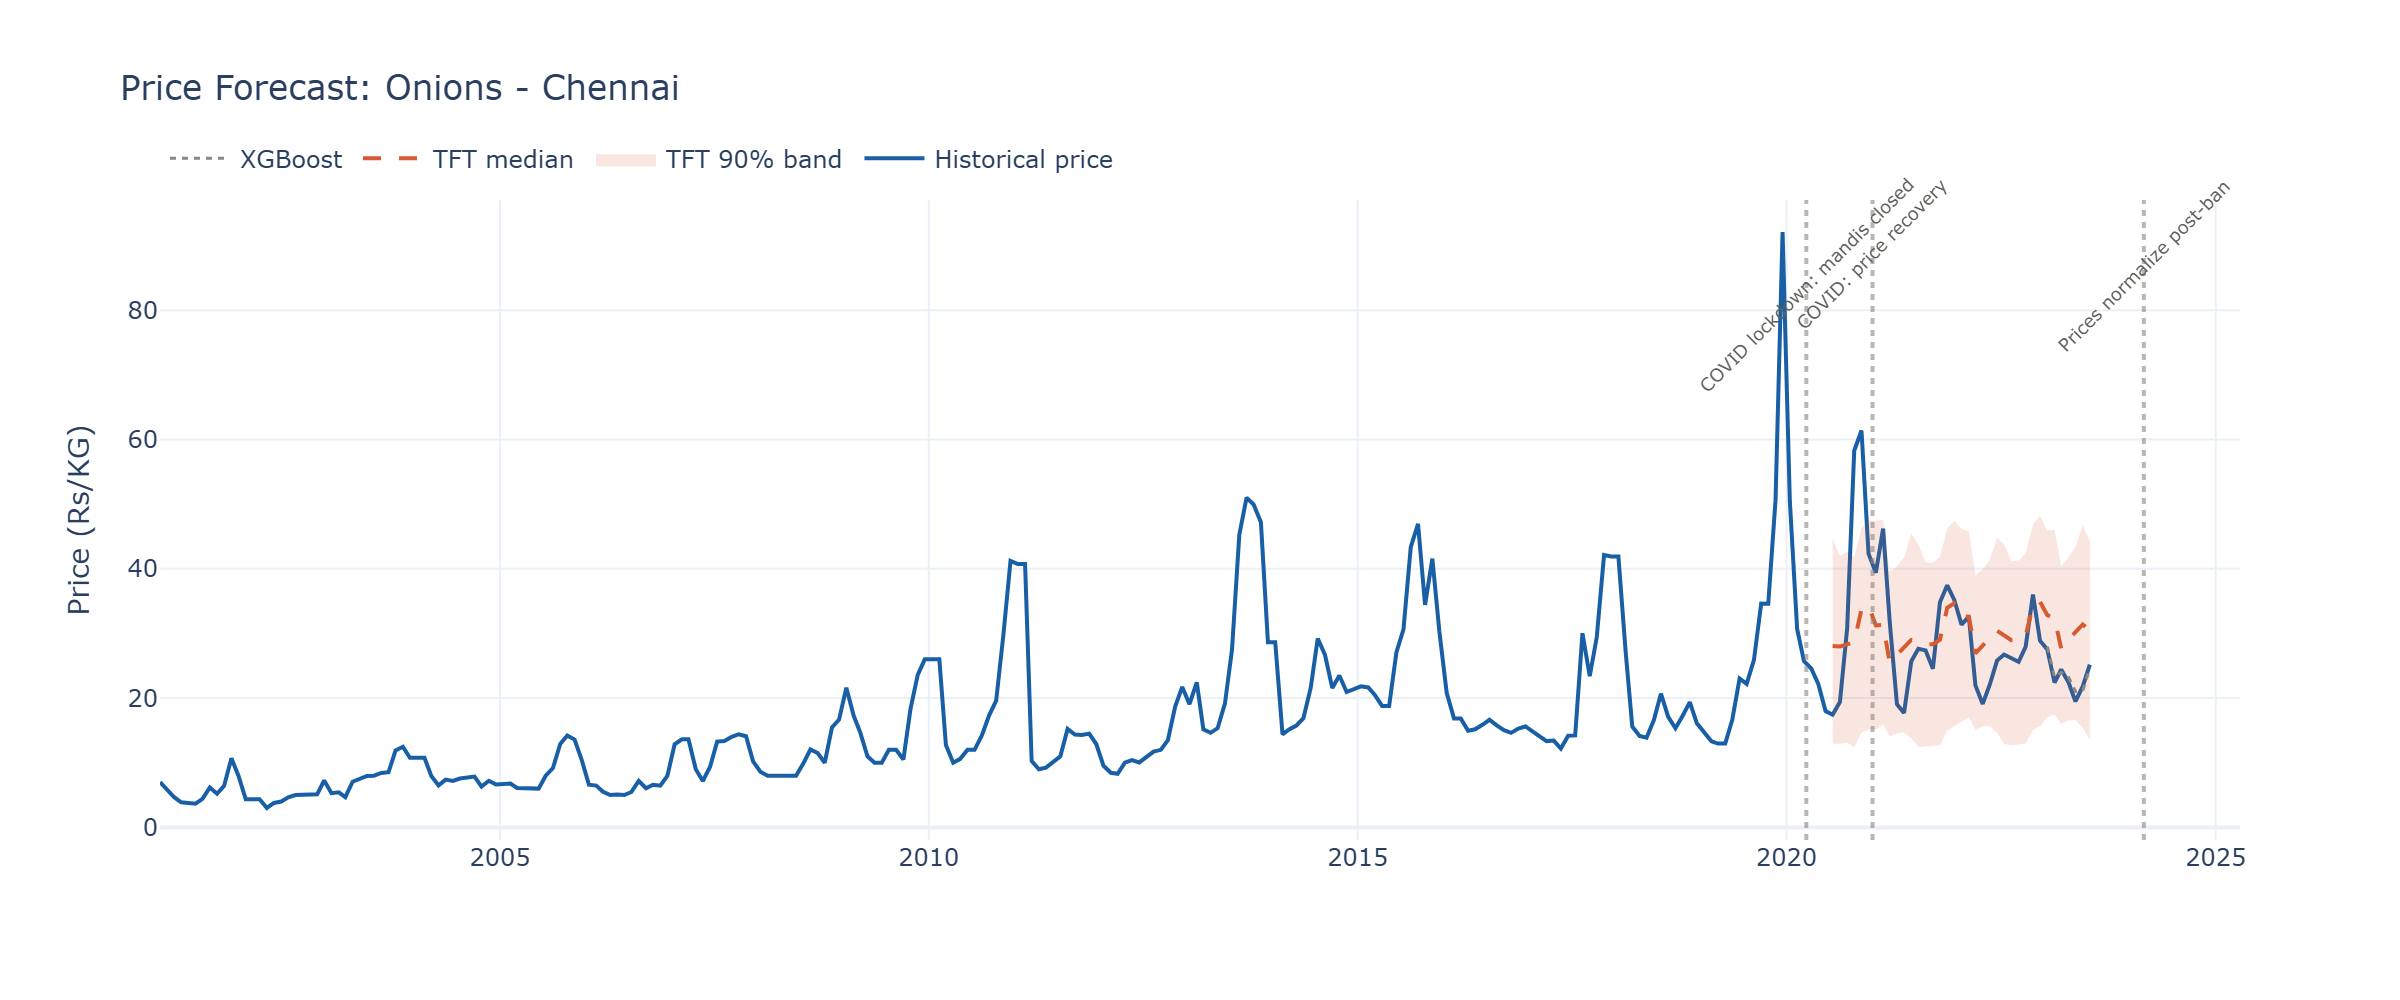
\includegraphics[width=0.88\textwidth]{figures/paper/quantile_forecast_onions.png}
\caption{TFT-XGBFusion-CQR calibrated prediction range (shaded) and median forecast (line)
versus actual onion prices on the held-out 2023 test set.}
\label{fig:ch6_qf_onions}
\end{figure}

\begin{figure}[H]
\centering
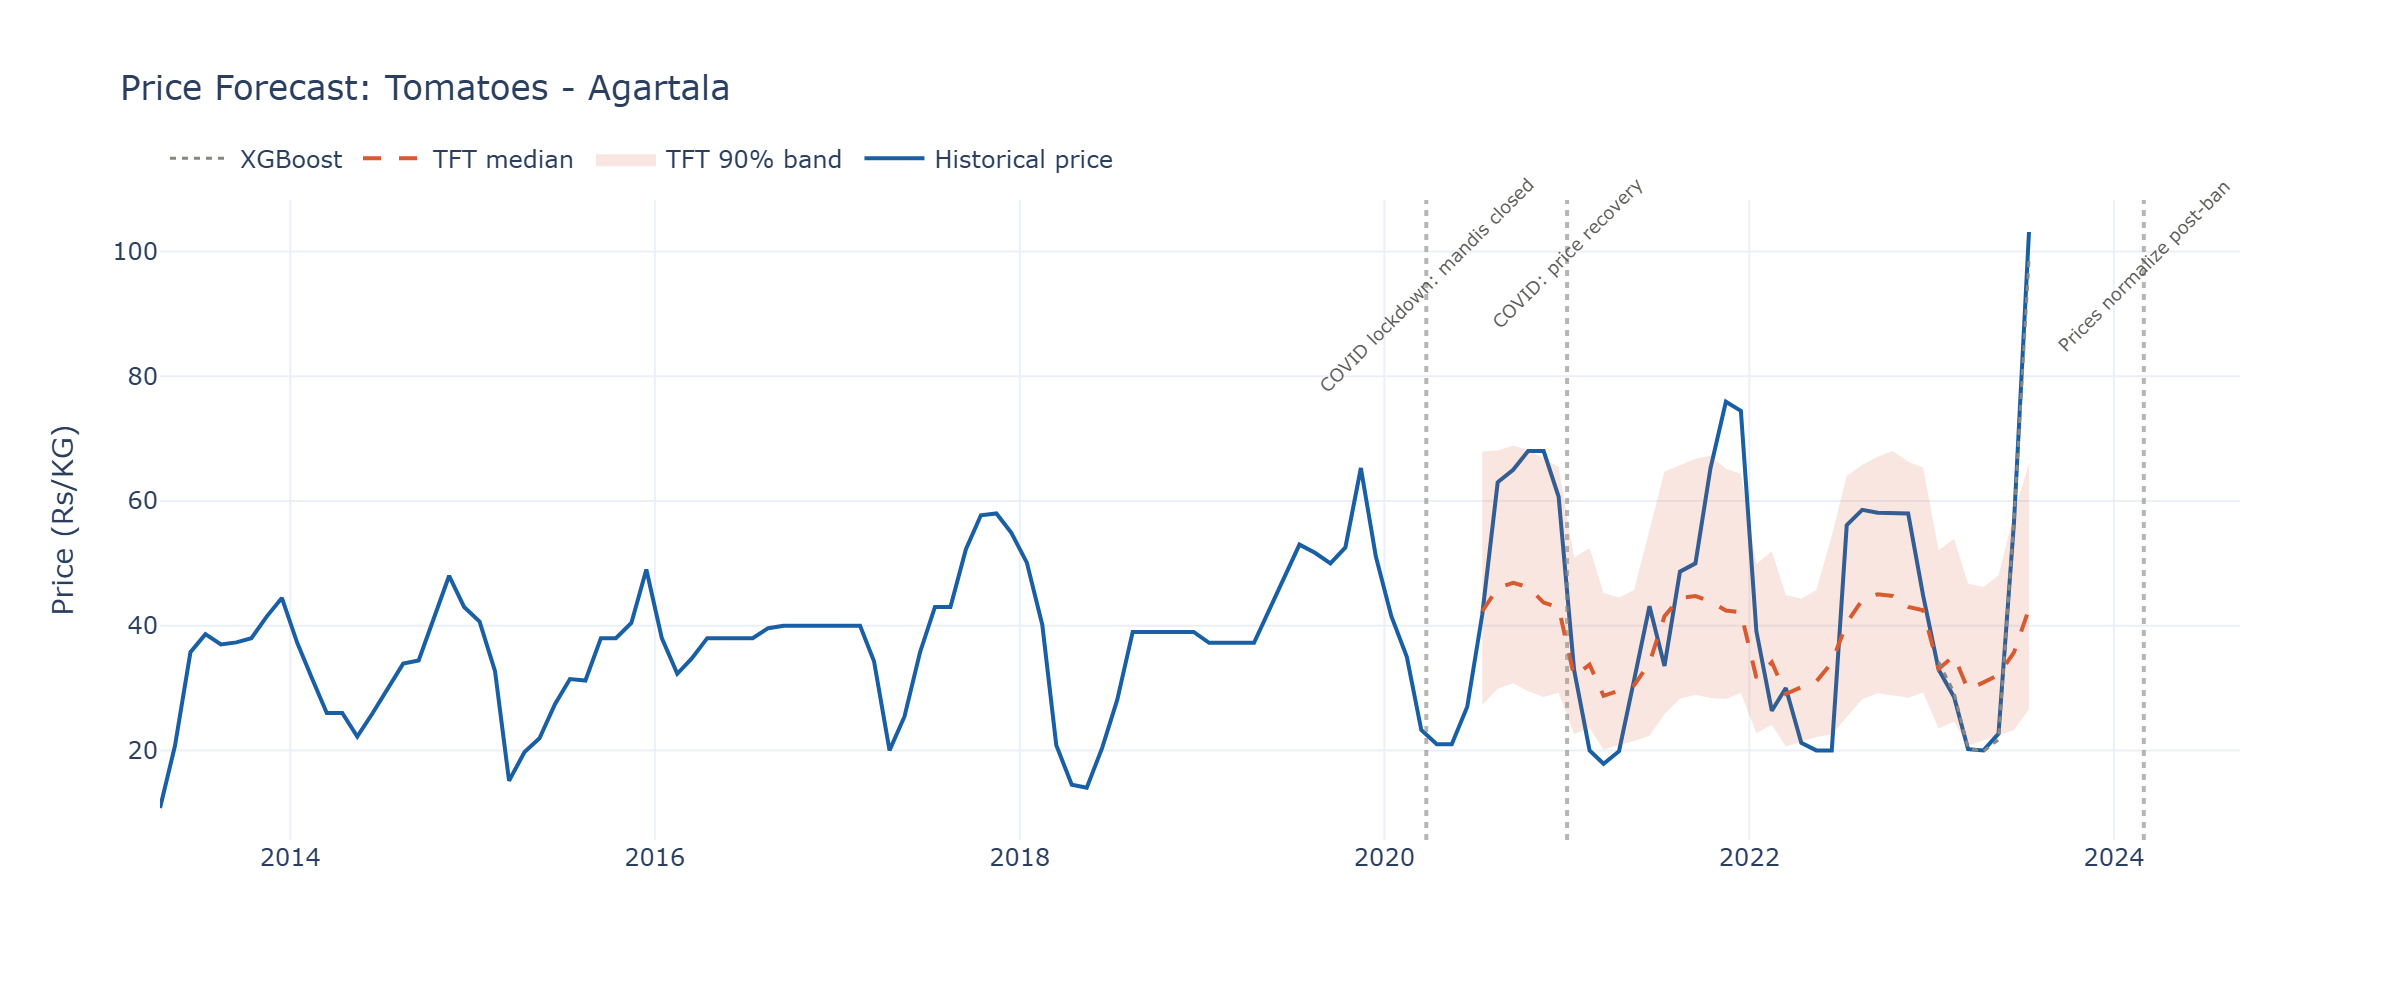
\includegraphics[width=0.88\textwidth]{figures/paper/quantile_forecast_tomatoes.png}
\caption{TFT-XGBFusion-CQR calibrated prediction range (shaded) and median forecast (line)
versus actual tomato prices on the held-out 2023 test set. The band correctly widens
during the mid-2023 price spike.}
\label{fig:ch6_qf_tomatoes}
\end{figure}

\begin{figure}[H]
\centering
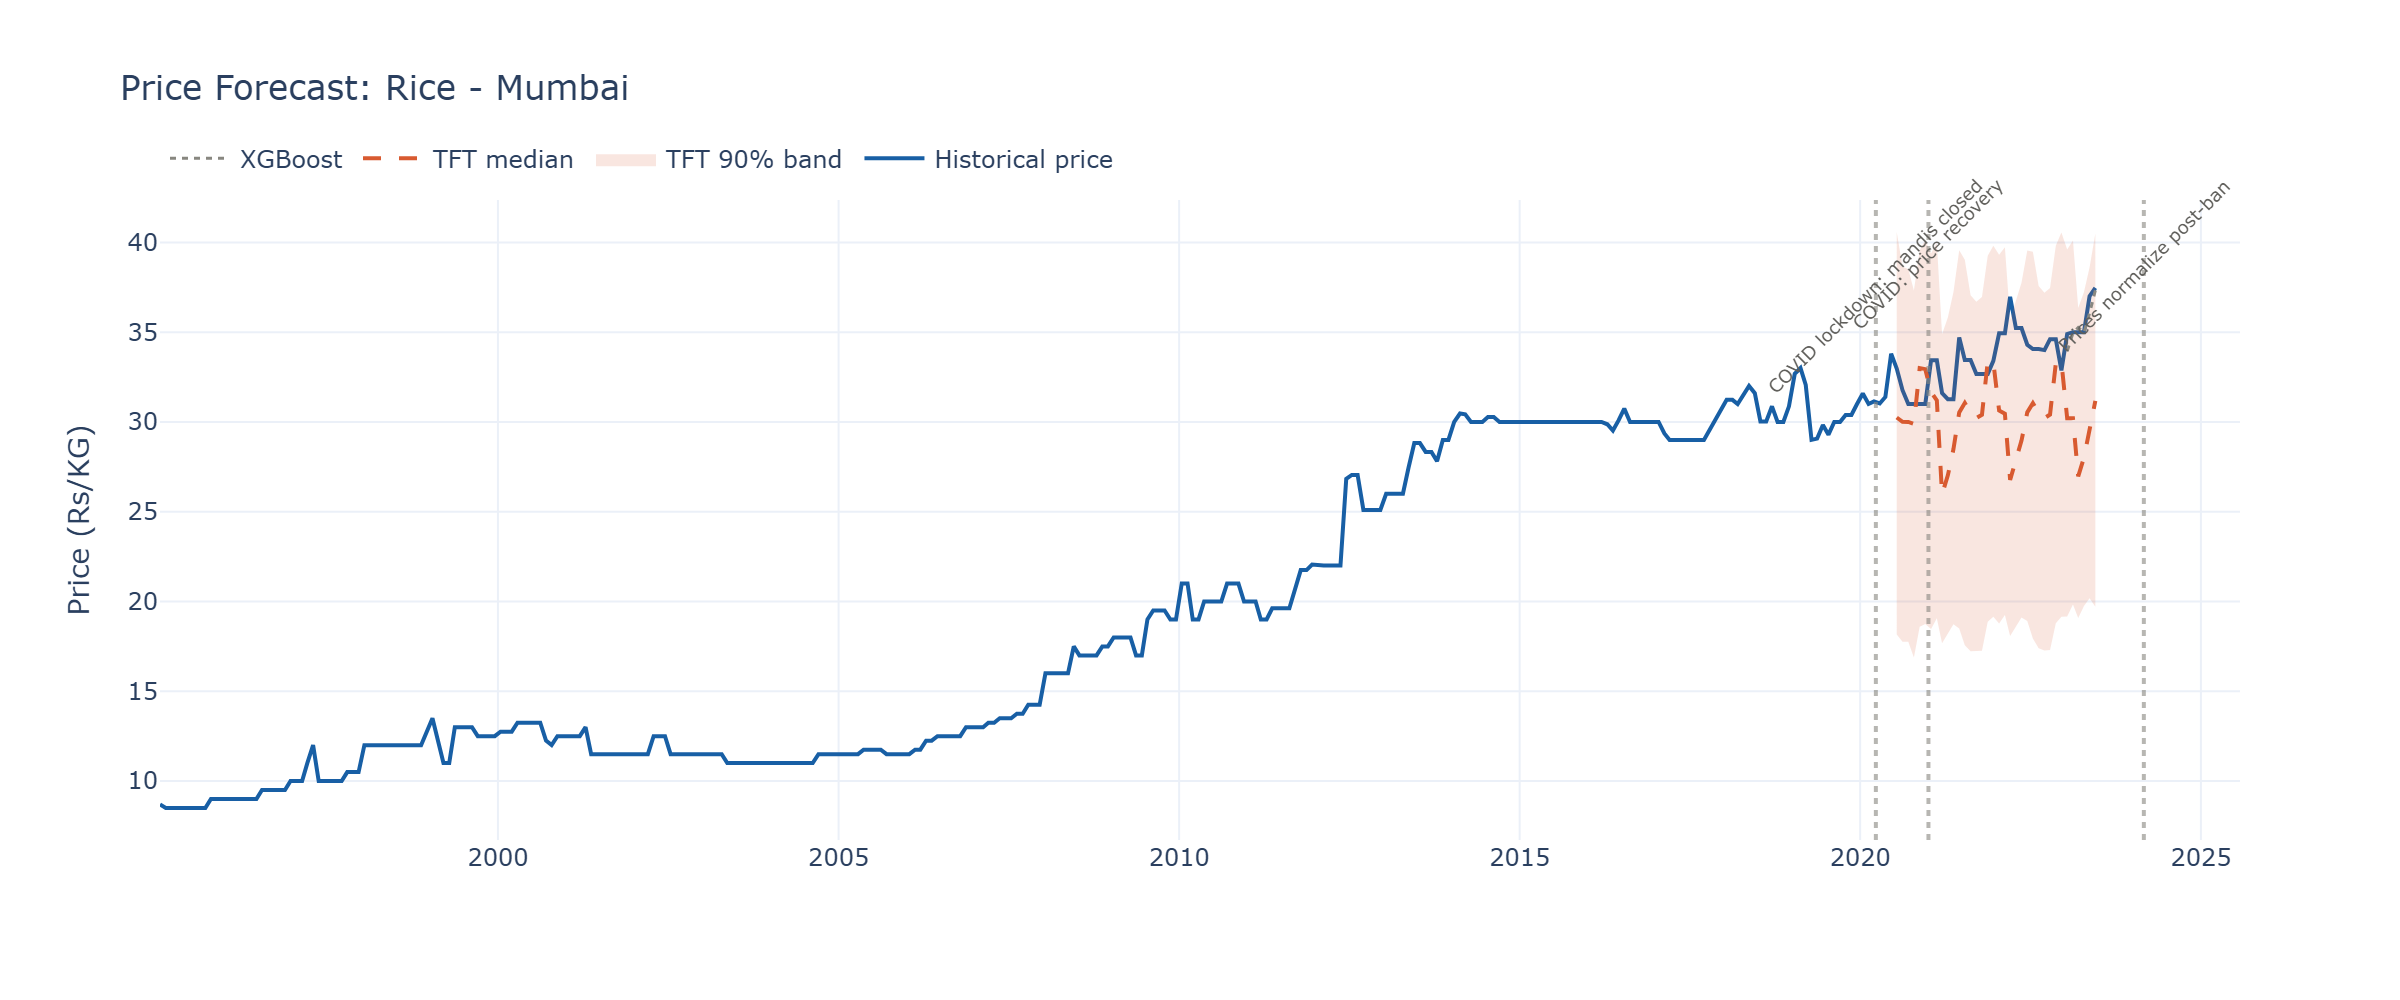
\includegraphics[width=0.88\textwidth]{figures/paper/quantile_forecast_rice.png}
\caption{TFT-XGBFusion-CQR calibrated prediction range (shaded) and median forecast (line)
versus actual rice prices on the held-out 2023 test set. Rice shows the tightest intervals
reflecting its stable price regime.}
\label{fig:ch6_qf_rice}
\end{figure}
Tomato is the most challenging crop. Its 2023 price spike, driven by supply disruptions not
visible in 24 months of price and weather history, compresses into monthly averages. The
82.5 percent coverage shows CQR absorbing most spike risk through wider intervals. Onions
achieve 90.9 percent coverage because monsoon driven shocks align well with the weather
features. Rice's 79.1 percent coverage marginally falls short of the 80 percent target,
indicating that the CQR offset slightly under-covers the rice distribution tail.

\section{Comparison with Literature}

\begin{table}[H]
\centering
\caption{Indicative comparison against selected published results}
\label{tab:ch6_litcompare}
\small
\begin{tabularx}{\textwidth}{L{0.28\textwidth}L{0.16\textwidth}L{0.20\textwidth}X}
\toprule
\textbf{Study} & \textbf{Target} & \textbf{Reported metric} & \textbf{Note} \\
\midrule
Nayak et al.\ (2024)   & Onion  & NBEATSX sMAPE 11.25\%    & Weekly; no uncertainty \\
Manogna et al.\ (2025) & Onion  & RNN MAPE 14.59\%          & Daily multi-market \\
Paul et al.\ (2022)    & Brinjal & GRNN MAPE 3.68--17.86\% & Market range; one crop \\
\textbf{This work}     & Onion  & MAPE 9.1\%               & Monthly; calibrated bands and interpretability \\
\bottomrule
\end{tabularx}
\end{table}

These values are not directly comparable because frequency and dataset scope differ across
studies. The onion MAPE of 9.1 percent on monthly data is competitive with weekly-data deep
models in recent literature, while additionally providing calibrated uncertainty bands and
statistically validated interpretable feature rankings.

\section{Key Observations}

\begin{itemize}
    \item XGBoost provides the strongest point accuracy and should not be dismissed as a
    baseline; its 1.58 Rs per kg MAE reflects how informative monthly lag features are.

    \item CQR calibration is essential: TFT-Base's 64.9 percent raw coverage is far below
    the 80 percent expectation and makes the model unsuitable as a risk-facing decision tool.

    \item The XGBoost fusion design is the most effective single intervention: injecting
    a clean XGBoost signal as a known covariate simultaneously improves point accuracy
    and narrows calibrated intervals.

    \item VSN feature rankings are stable (Kendall $\tau = 0.942$) and can be treated as
    model-internal attribution signals, though they do not constitute causal proof of
    any relationship between weather and price.

    \item Tomatoes remain the hardest crop across all metrics, representing the strongest
    case for incorporating supply-event covariates in future work.
\end{itemize}

%% =====================================================================
\chapter{Implementation and Dashboard}
%% =====================================================================

\section{Technology Stack}

\begin{table}[H]
\centering
\caption{Core implementation stack}
\label{tab:ch7_stack}
\small
\begin{tabularx}{\textwidth}{L{0.28\textwidth}L{0.28\textwidth}X}
\toprule
\textbf{Layer} & \textbf{Technology} & \textbf{Purpose} \\
\midrule
Data engineering     & pandas, numpy              & Filtering, joins, feature generation \\
Weather ingestion    & requests + NASA POWER API  & Monthly exogenous covariate acquisition \\
Deep forecasting     & PyTorch, PyTorch Forecasting, Lightning & TFT training and inference \\
Baseline modeling    & XGBoost + joblib           & Point forecast and artifact serialization \\
Evaluation and plots & Plotly, Kaleido            & Metrics and visualisation generation \\
Application layer    & Streamlit                  & Interactive forecast and explainability dashboard \\
\bottomrule
\end{tabularx}
\end{table}

Training was run on an NVIDIA GPU (CUDA 12.8). Each TFT family takes 30 to 90 minutes on
GPU and 4 to 8 hours on CPU. Dashboard inference runs on CPU in real time with artifact
loading times under two seconds.

\section{Dashboard Views}

The Streamlit dashboard exposes four views accessible through a sidebar crop-market selector.

\begin{itemize}
    \item \textbf{Price Forecast:} Historical price series overlaid with TFT-XGBFusion-CQR
    median and the calibrated $q_{0.1}$--$q_{0.9}$ band. Vertical markers flag months where
    the relative price change exceeds 25 percent. An optional XGBoost overlay enables direct
    comparison of probabilistic and point forecasts on the same chart.

    \item \textbf{Future Forecast:} Month-by-month projection cards for the next six months,
    each showing the predicted median, the calibrated interval, and a risk classification
    (Stable, Moderate, or High) derived from the relative interval width
    $r_t = (q_{0.9,t} - q_{0.1,t})\,/\,q_{0.5,t}$.

    \item \textbf{Explainability:} XGBoost feature importances, TFT encoder and decoder VSN
    weight bar charts, and a temporal attention heatmap showing which past months the model
    attended to most. Weather variables consistently dominate encoder importance, consistent
    with the bootstrap result.

    \item \textbf{Present vs Predicted:} Test-period chart comparing actual prices to TFT
    predictions, alongside a per-metric summary table (MAE, RMSE, MAPE, coverage, band
    width). Enables operational validation without re-running the evaluation pipeline.
\end{itemize}

\begin{figure}[H]
\centering
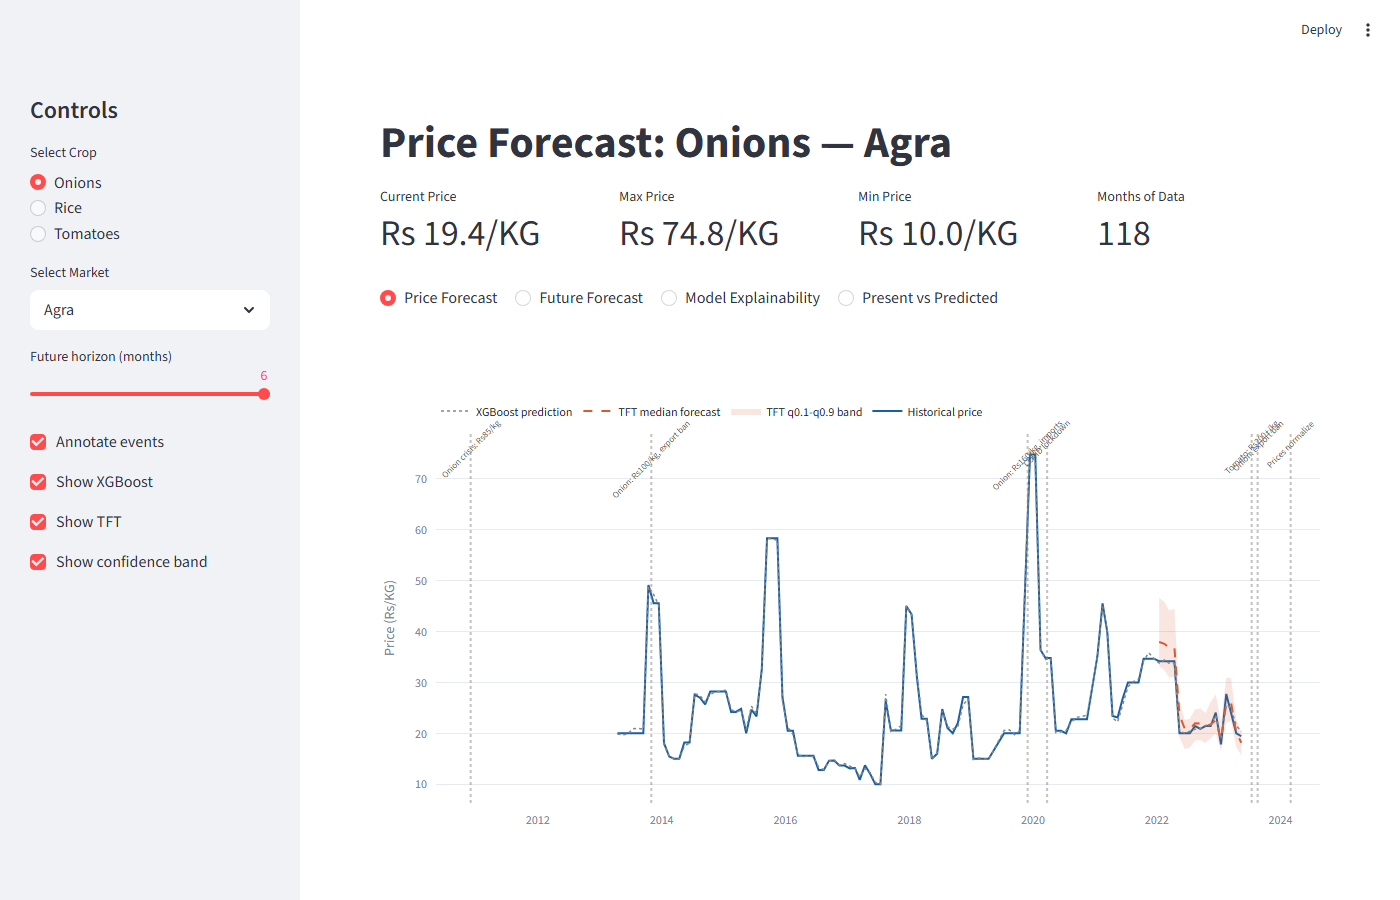
\includegraphics[width=0.85\textwidth]{figures/dashboard_view1_forecast.png}
\caption{Dashboard Price Forecast view: historical prices overlaid with the
TFT-XGBFusion-CQR median forecast and calibrated uncertainty band.}
\label{fig:dash_forecast}
\end{figure}

\begin{figure}[H]
\centering
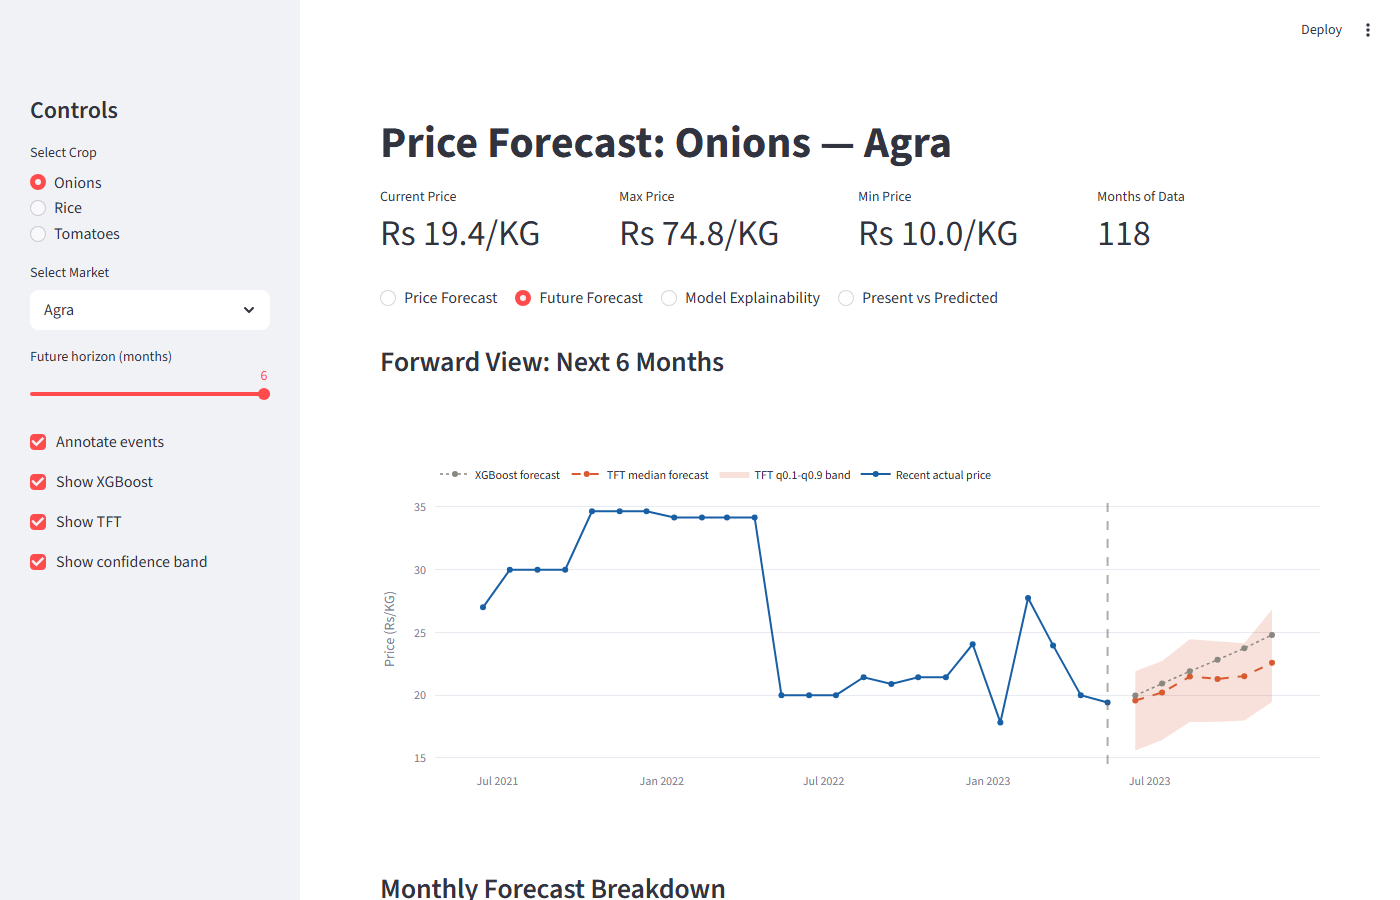
\includegraphics[width=0.85\textwidth]{figures/dashboard_view2_future.png}
\caption{Dashboard Future Forecast view: month-by-month projection cards for the next six
months with predicted median, calibrated interval, and risk classification.}
\label{fig:dash_future}
\end{figure}

\begin{figure}[H]
\centering
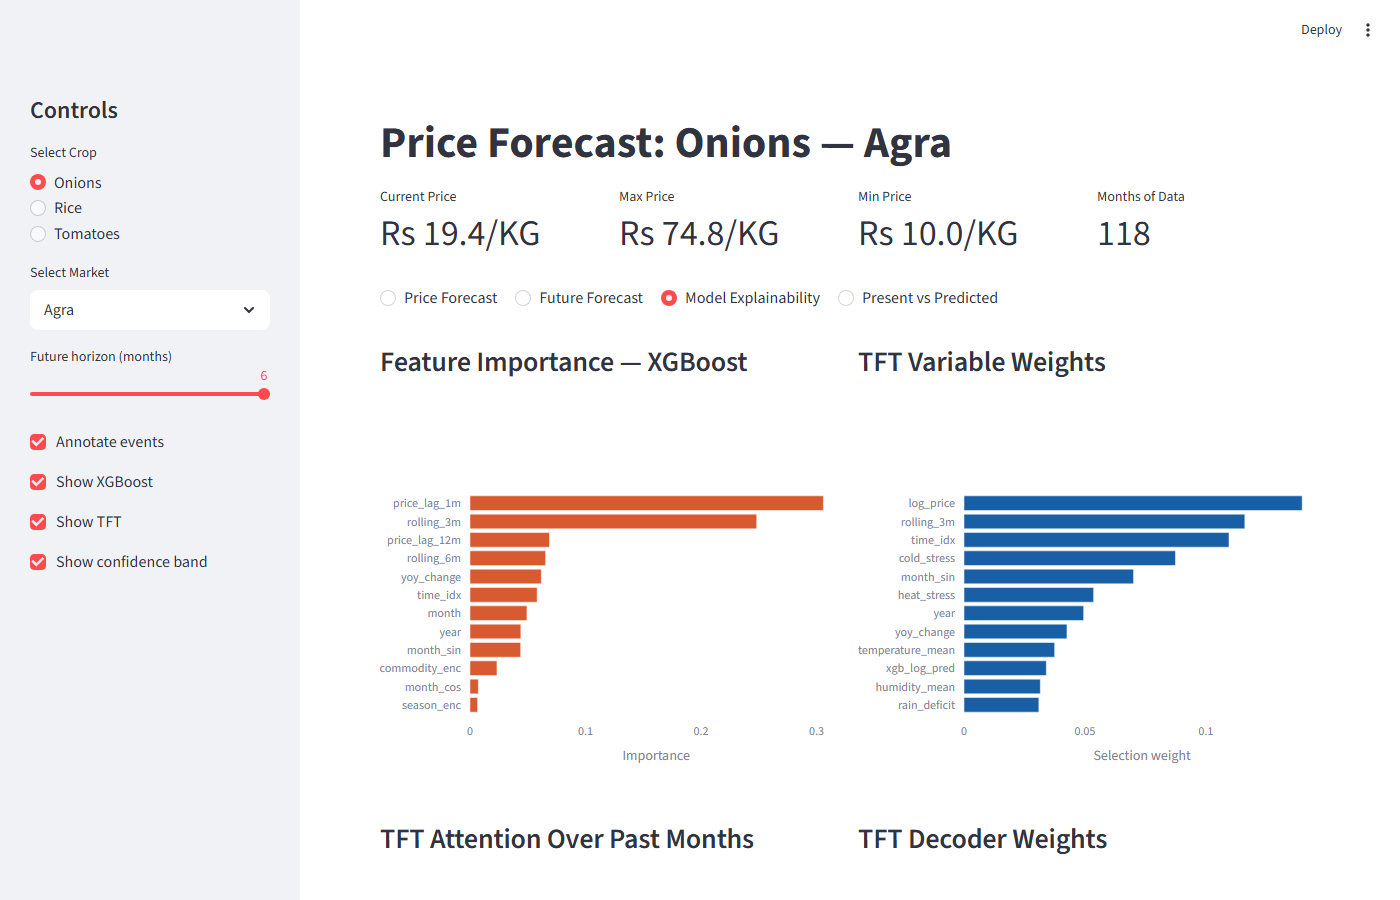
\includegraphics[width=0.85\textwidth]{figures/dashboard_view3_explainability.png}
\caption{Dashboard Explainability view: XGBoost gain-based feature importances (top), TFT
encoder and decoder VSN weights (middle), and temporal attention heatmap (bottom).}
\label{fig:dash_explain}
\end{figure}

\begin{figure}[H]
\centering
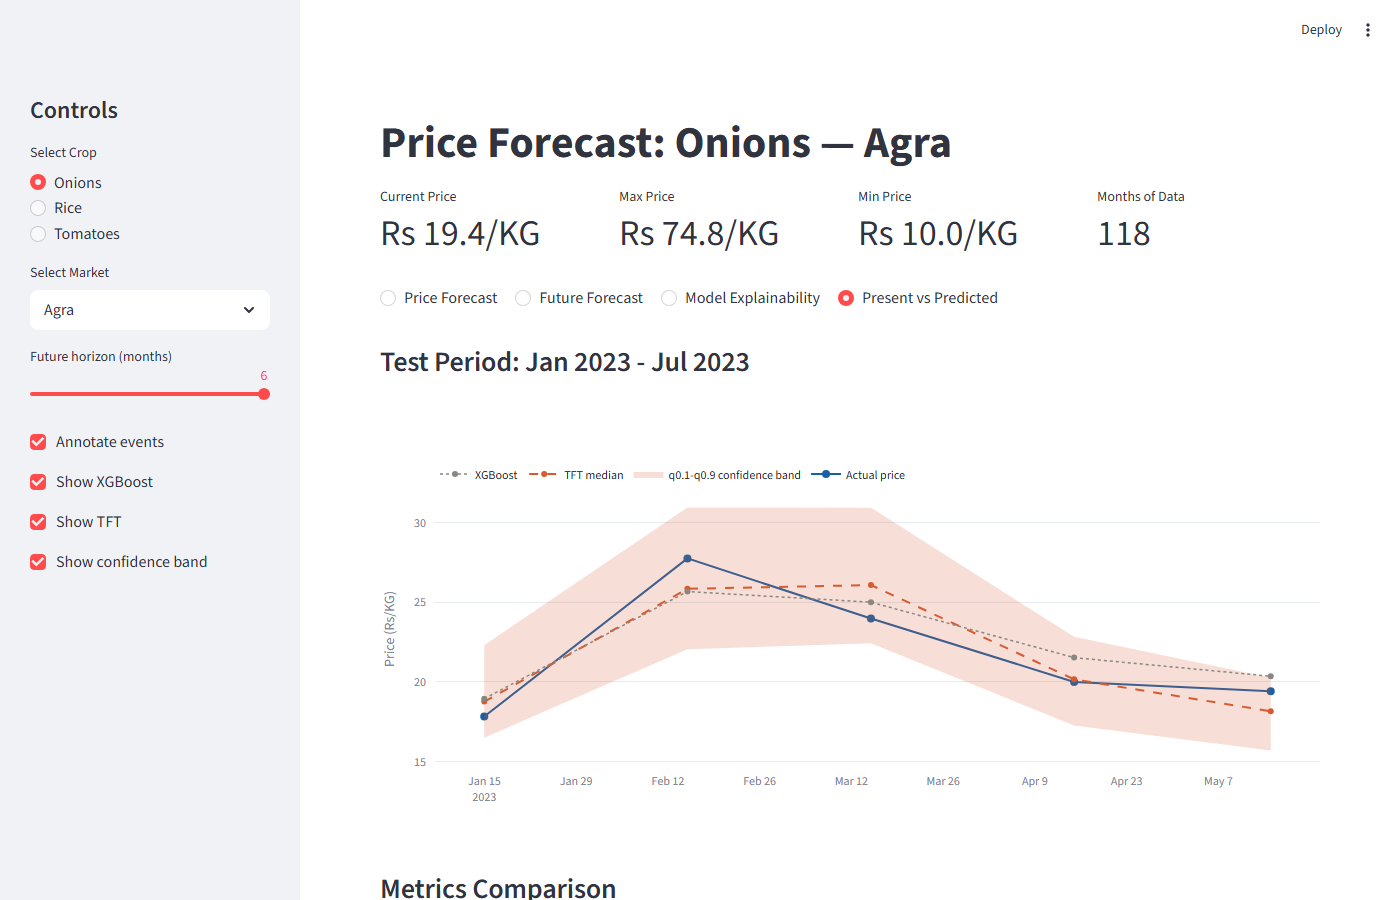
\includegraphics[width=0.85\textwidth]{figures/dashboard_view4_evaluation.png}
\caption{Dashboard Present vs Predicted view: actual prices overlaid on model predictions
for the 2023 held-out test period with the calibrated band as a shaded region.}
\label{fig:dash_eval}
\end{figure}

\section{Model Cascade Selection}

At startup, the application checks which TFT artifacts are available on disk. If the fused
checkpoint and dataset are present, it selects TFT-XGBFusion-CQR as the active probabilistic
model. If not present, it falls back to TFT-Retrain21-CQR, and then to TFT-Base. CQR
calibration offsets are loaded from the corresponding \texttt{conformal\_offsets\_*.json}
file. This cascading selection means the dashboard always uses the best available model
without requiring manual configuration.

%% =====================================================================
\chapter{Conclusion and Future Work}
%% =====================================================================

\section{Conclusion}

This mini project built an interpretable, uncertainty-aware crop price forecasting system
for Indian markets. The system covers three crops (onions, tomatoes, rice) across 53 markets
in a monthly panel spanning 1994 to 2026, and delivers probabilistic forecasts with
calibrated uncertainty bands and statistically validated interpretable feature attribution.

Among all model families evaluated, TFT-XGBFusion-CQR provides the strongest practical
balance: an MAE of 5.27 Rs per kg, a MAPE of 11.4 percent, and 84.0 percent empirical
coverage on the 2023 test window. Paired statistical tests ($p = 4.6 \times 10^{-86}$,
Cohen's $d = -0.79$) and bootstrap VSN stability analysis (Kendall $\tau = 0.942$) confirm
that the improvements are consistent and not artifacts of random variation.

XGBoost remains the strongest pure point model but does not provide calibrated uncertainty
or interpretable temporal reasoning. The deployed Streamlit dashboard operationalises the
broader objective: actionable crop price forecasting with quantified risk and inspectable
model reasoning, in one reproducible workflow.

\section{Future Work}

\begin{enumerate}
    \item \textbf{News and event integration.} The dashboard already fetches commodity news
    for qualitative context. The direct next step is building a pipeline to ingest news
    headlines, apply commodity-specific sentiment scoring, and inject the resulting signal
    as an exogenous TFT covariate. This is the most targeted fix for tomato's abrupt
    2023-type spikes.

    \item \textbf{Richer supply-side covariates.} Adding market arrivals from AGMARKNET,
    export ban episodes, cold storage capacity, and fuel price index would address the
    largest identified gap in the current feature set. These policy and logistics variables
    drove both the 2019 onion and 2023 tomato episodes.

    \item \textbf{Rolling conformal recalibration.} Static CQR offsets are computed from a
    fixed historical validation window. A rolling recalibration that updates offsets as new
    data arrives would adapt to regime shifts faster, particularly for tomato markets.

    \item \textbf{Higher-frequency expansion.} Weekly or daily price data from AGMARKNET
    would multiply the training set size, improve short-term spike detection, and allow
    shorter recalibration windows. The current monthly framework is a practical starting
    point, not a fundamental constraint.

    \item \textbf{Broader crop and market coverage.} Expanding to pulses, spices, and
    edible oils, and extending to more state-level mandi data, would increase utility for
    national agricultural policy monitoring. External validation on post-2024 data is also
    needed before production deployment.
\end{enumerate}

%% =====================================================================
\chapter*{Bibliography}
\addcontentsline{toc}{chapter}{Bibliography}
%% =====================================================================

\begin{enumerate}
    \item Lim, B., Arik, S.~O., Loeff, N., and Pfister, T. (2021). Temporal Fusion
    Transformers for Interpretable Multi-horizon Time Series Forecasting.
    \textit{International Journal of Forecasting}, 37(4), 1748--1764.

    \item Romano, Y., Patterson, E., and Candes, E. (2019). Conformalized Quantile
    Regression. \textit{Advances in Neural Information Processing Systems (NeurIPS)}.

    \item Nayak, G.~H.~H., Alam, M.~W., Singh, K.~N., et al. (2024). Exogenous Variable
    Driven Deep Learning Models for Improved Price Forecasting of TOP Crops in India.
    \textit{Scientific Reports}.

    \item Manogna, R.~L., Dharmaji, V., and Sarang, S. (2025). Enhancing Agricultural
    Commodity Price Forecasting with Deep Learning. \textit{Scientific Reports}.

    \item Paul, R.~K., Yeasin, M., et al. (2022). Machine Learning Techniques for
    Forecasting Agricultural Prices: A Case of Brinjal in Odisha, India. \textit{PLOS ONE}.

    \item Box, G.~E.~P. and Jenkins, G.~M. (2015). Time Series Analysis: Forecasting and
    Control, 5th ed. John Wiley and Sons, Hoboken, NJ.

    \item Wolpert, D.~H. (1992). Stacked generalization. \textit{Neural Networks},
    5(2), 241--259.

    \item World Food Programme (2026 access). WFP Food Prices for India Dataset.
    \url{https://data.humdata.org/dataset/wfp-food-prices-for-india}.

    \item NASA POWER Project (2026 access). Monthly Point API.
    \url{https://power.larc.nasa.gov}.

    \item PyTorch Forecasting Documentation (2026 access).
    \url{https://pytorch-forecasting.readthedocs.io}.

    \item PyTorch Lightning Documentation (2026 access).
    \url{https://lightning.ai/docs/pytorch}.

    \item Streamlit Documentation (2026 access). \url{https://docs.streamlit.io}.
\end{enumerate}

\end{document}
